% =====================================================================
%  Taiwanese Bankruptcy Prediction — final report (Augmented Decision)
%  Compile from this folder:   tectonic main.tex      (or: xelatex main.tex, twice)
%  Figures in figures/ are exported by:  .venv/bin/python slides/make_figures.py "IBM Plex Sans"
% =====================================================================
\documentclass[11pt,a4paper]{article}

% ---------- Page and fonts ----------
\usepackage[a4paper, top=24mm, bottom=26mm, left=25mm, right=25mm, headsep=8mm]{geometry}
\usepackage{fontspec}
\setmainfont{IBMPlexSerif}[Extension=.otf, UprightFont=*-Regular, BoldFont=*-SemiBold, ItalicFont=*-Italic, Scale=0.94]
\setsansfont{IBMPlexSans}[Extension=.otf, UprightFont=*-Regular, BoldFont=*-SemiBold, ItalicFont=*-Italic, BoldItalicFont=*-SemiBoldItalic]
\setmonofont{IBMPlexMono}[Extension=.otf, UprightFont=*-Regular, BoldFont=*-SemiBold, ItalicFont=*-Italic, Scale=0.86]
\linespread{1.12}
\setlength{\emergencystretch}{2em}

\usepackage{amsmath, amssymb}
\usepackage{xcolor, graphicx, booktabs, tabularx, enumitem, listings, caption}
\usepackage[section]{placeins}
\usepackage{titlesec, fancyhdr}
\usepackage{tikz, pgfplots}
\usepackage{array, calc}                 % tables rendered by pandoc in the appendix
\usepackage[most]{tcolorbox}
\usepackage[normalem]{ulem}
\usepackage{fvextra, needspace}                     % code blocks of the appendix wrap long lines
\usetikzlibrary{positioning, arrows.meta}
\pgfplotsset{compat=1.18}
\graphicspath{{figures/}}

% ---------- Palette (same as the slides) ----------
\definecolor{paper}{HTML}{F6F3EC}
\definecolor{ink}{HTML}{16181D}
\definecolor{muted}{HTML}{6B6F78}
\definecolor{rule}{HTML}{D9D2C5}
\definecolor{risk}{HTML}{B42318}
\definecolor{model}{HTML}{155E63}
\definecolor{bench}{HTML}{B8862B}
\definecolor{risktint}{HTML}{F2DAD6}
\definecolor{modeltint}{HTML}{D5E5E3}
\definecolor{card}{HTML}{FFFEFB}
\color{ink}

\usepackage[colorlinks=true, linkcolor=model, urlcolor=model, citecolor=model]{hyperref}

% ---------- Headings, header, captions, lists ----------
\titleformat{\section}{\sffamily\Large\bfseries}{\color{risk}\thesection}{0.7em}{}
\titleformat{\subsection}{\sffamily\large\bfseries}{\color{risk}\thesubsection}{0.7em}{}
\titleformat{\paragraph}[runin]{\sffamily\bfseries}{}{}{}[.]
\titlespacing*{\section}{0pt}{5mm}{2.5mm}
\titlespacing*{\subsection}{0pt}{4mm}{1.8mm}
\newcommand{\caps}[1]{{\sffamily\fontsize{7.5}{9}\selectfont\addfontfeatures{LetterSpace=12}#1}}

\pagestyle{fancy}
\fancyhf{}
\renewcommand{\headrulewidth}{0pt}
\fancyhead[L]{\color{muted}\caps{TAIWANESE BANKRUPTCY PREDICTION}}
\fancyhead[R]{\color{muted}\caps{AUGMENTED DECISION \enspace·\enspace FINAL REPORT}}
\fancyfoot[C]{\sffamily\small\color{muted}\thepage}

\captionsetup{font={small,sf}, labelfont={bf,color=risk}, labelsep=period, skip=5pt}
\setlist[itemize]{leftmargin=1.3em, itemsep=1.5pt, topsep=3pt, label={\color{risk}\rule[0.33ex]{0.6em}{0.9pt}}}
\setlist[enumerate]{leftmargin=1.5em, itemsep=1.5pt, topsep=3pt, label={\color{risk}\sffamily\bfseries\arabic*}}
\tikzset{every picture/.append style={font=\sffamily}}
\newcommand{\tablefont}{\sffamily\small}
\renewcommand{\arraystretch}{1.18}

% ---------- Code snapshots ----------
\lstdefinestyle{nb}{language=Python, basicstyle=\ttfamily\footnotesize, columns=fullflexible, keepspaces=true,
  keywordstyle=\color{model}\bfseries, stringstyle=\color{risk}, commentstyle=\color{muted}\itshape,
  backgroundcolor=\color{paper}, frame=leftline, framerule=1.6pt, rulecolor=\color{risk},
  xleftmargin=4mm, framexleftmargin=4mm, aboveskip=6pt, belowskip=4pt, showstringspaces=false,
  morekeywords={True, False, None}}
\lstset{style=nb}
\renewcommand{\lstlistingname}{Code}

% ---------- Appendix: rendered Markdown files and verbatim prompt log ----------
\providecommand{\tightlist}{\setlength{\itemsep}{0pt}\setlength{\parskip}{0pt}}
\providecommand{\st}[1]{\sout{#1}}
\newcommand{\mdh}[2]{% Markdown headings inside a rendered file
  \par\needspace{5\baselineskip}% keep a heading with the start of its content
  \ifcase#1\or \medskip{\sffamily\large\bfseries #2}\par\smallskip
  \or \medskip{\sffamily\normalsize\bfseries\color{risk}#2}\par\smallskip
  \else \smallskip{\sffamily\small\bfseries #2}\par \fi}
\newtcolorbox{mdfile}[2]{enhanced, breakable, colback=card, colframe=rule, boxrule=0.4pt, arc=1.5pt,
  borderline west={1.8pt}{0pt}{risk}, colbacktitle=paper, coltitle=ink, fonttitle=\sffamily\small,
  title={\ttfamily #1\hfill\sffamily\color{muted}#2}, before upper={\small},
  left=4mm, right=4mm, top=2mm, bottom=2mm, before skip=3mm, after skip=5mm}
\newcommand{\promptentry}[4]{% number, phase, time, verbatim text
  \par\noindent\begin{minipage}[t]{17mm}{\sffamily\small\bfseries\color{risk}\##1}\\{\sffamily\scriptsize\color{muted}#2}\end{minipage}%
  \begin{minipage}[t]{\linewidth-17mm}{\sffamily\scriptsize\color{muted}#3}\\[0.3mm]{\small #4}\end{minipage}\par\vspace{2.2mm}}

\begin{document}

% =====================================================================
%  TITLE BLOCK
% =====================================================================
\thispagestyle{empty}
\begin{tikzpicture}[remember picture, overlay]
  \fill[risk] ([yshift=-24mm]current page.north west) rectangle ++(3mm,-3mm);
\end{tikzpicture}%
{\color{risk}\caps{AUGMENTED DECISION \quad·\quad FINAL PROJECT REPORT}}\par\vspace{5mm}
{\fontsize{25}{30}\selectfont Flagging bankruptcy \textit{before} it happens}\par\vspace{3mm}
{\sffamily\large\color{muted} Cost-sensitive screening of Taiwanese firms\\ with LASSO selection and a decision tree}\par\vspace{5mm}
{\sffamily\bfseries Yassine ERRAJI \enspace·\enspace William PELTIER \enspace·\enspace Ben DAESH \enspace·\enspace Simon AMAR}\par\vspace{1mm}
{\sffamily\small\color{muted} 23 October 2026 \enspace·\enspace Code: \href{https://github.com/yassineerraji/Augmented-Decision-Final-Project}{github.com/yassineerraji/Augmented-Decision-Final-Project}}\par\vspace{5mm}

\noindent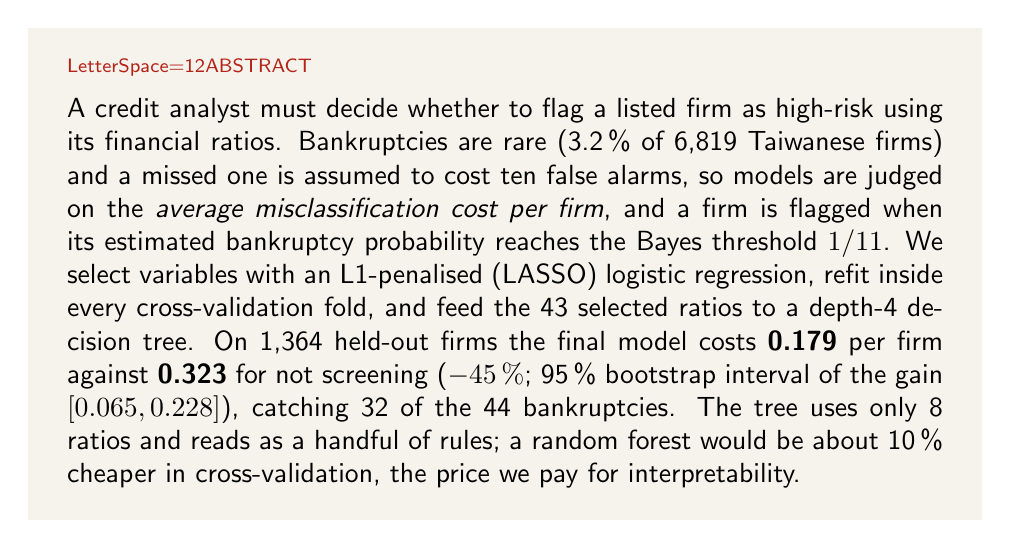
\begin{tikzpicture}
  \node[fill=paper, inner xsep=5mm, inner ysep=4mm, text width=\linewidth-10mm, align=justify] {%
    {\color{risk}\caps{ABSTRACT}}\par\vspace{1.5mm}
    A credit analyst must decide whether to flag a listed firm as high-risk using its financial ratios. Bankruptcies are rare (3.2\,\% of 6,819 Taiwanese firms) and a missed one is assumed to cost ten false alarms, so models are judged on the \emph{average misclassification cost per firm}, and a firm is flagged when its estimated bankruptcy probability reaches the Bayes threshold $1/11$. We select variables with an L1-penalised (LASSO) logistic regression, refit inside every cross-validation fold, and feed the 43 selected ratios to a depth-4 decision tree. On 1,364 held-out firms the final model costs \textbf{0.179} per firm against \textbf{0.323} for not screening ($-45\,\%$; 95\,\% bootstrap interval of the gain $[0.065, 0.228]$), catching 32 of the 44 bankruptcies. The tree uses only 8 ratios and reads as a handful of rules; a random forest would be about 10\,\% cheaper in cross-validation, the price we pay for interpretability.};
\end{tikzpicture}

% =====================================================================
\section{Problem formulation}
% =====================================================================

\paragraph{Decision and target} A credit analyst reviews a listed firm and chooses between two actions: \emph{flag} it as high-risk (deny or reprice credit, open a closer review) or \emph{do not flag} it. The target is $Y = $ \texttt{Bankrupt?}, equal to 1 if the firm went bankrupt under the Taiwan Stock Exchange rules. The inputs $x$ are 95 financial ratios, assumed to be known before the outcome.

\paragraph{Loss and decision rule} The two possible errors do not cost the same (Table~\ref{tab:loss}). With $p = P(Y=1 \mid x)$, flagging has expected cost $C_{FP}(1-p)$ and not flagging $C_{FN}\,p$, so the Bayes decision rule (Lecture~1) flags a firm when
\begin{equation}\label{eq:bayes}
  p \;\ge\; \frac{C_{FP}}{C_{FP}+C_{FN}} \;=\; \frac{1}{11} \;\approx\; 0.09 .
\end{equation}
The costs $C_{FN}=10$ and $C_{FP}=1$ are stipulated, not estimated; Section~\ref{sec:sensitivity} shows how the decisions change with the cost ratio.

\begin{table}[htbp]\centering\tablefont
  \caption{Loss table of the decision problem.}\label{tab:loss}
  \begin{tabular}{lcc}
    \toprule
    & Healthy firm ($Y=0$) & Bankrupt firm ($Y=1$) \\
    \midrule
    Do not flag ($a=0$) & 0 & $C_{FN} = 10$ \ (missed bankruptcy) \\
    Flag ($a=1$) & $C_{FP} = 1$ \ (false alarm) & 0 \\
    \bottomrule
  \end{tabular}
\end{table}

\paragraph{Metric and baseline} A model is scored by its empirical risk under the loss table, the \emph{average cost per firm} (lower is better), complemented by recall and precision:
\begin{equation}\label{eq:risk}
  \hat R_n \;=\; \frac{1}{n}\sum_{i=1}^{n} L(\hat a_i, y_i) \;=\; \frac{C_{FN}\cdot \mathrm{FN} + C_{FP}\cdot \mathrm{FP}}{n}.
\end{equation}
Accuracy is unsuitable: the majority-class rule ``never flag'' is 96.8\,\% accurate while catching no bankruptcy. That rule is our \textbf{baseline}; its cost is $10 \times 0.032 \approx 0.323$ per firm.

\paragraph{Data} The data come from the Taiwan Economic Journal for 1999–2009 and are distributed by the UCI Machine Learning Repository~\cite{uci, liang}. Table~\ref{tab:data} summarises them. Two features of the data shape our method. First, the ratios are highly redundant: 50 pairs have a Spearman correlation $|\rho| > 0.95$, involving 47 of the 94 usable ratios (Figure~\ref{fig:heatmap}). Second, 24 ratios mix values in $[0,1]$ with values between $6\times10^{5}$ and $10^{10}$, with nothing in between, which looks like an encoding artefact. The strongest single predictors are profitability ratios (EPS, net income to total assets, ROA), each with a univariate AUC between 0.86 and 0.89. This exploratory analysis is descriptive only; every modelling choice below is made on the training set.

\begin{table}[htbp]\centering\tablefont
  \caption{The dataset at a glance.}\label{tab:data}
  \begin{tabularx}{0.86\linewidth}{lX}
    \toprule
    Observations & 6,819 listed Taiwanese firms, 1999–2009 \\
    Variables & 95 financial ratios (one, \texttt{Net Income Flag}, is constant and is dropped: 94 remain) \\
    Target distribution & 220 bankrupt firms (3.2\,\%), 6,599 healthy firms \\
    Missing values, duplicates & none, none \\
    Preprocessing required & drop the constant column; handle 24 ratios with extreme values (Section~\ref{sec:preproc}) \\
    \bottomrule
  \end{tabularx}
\end{table}

\begin{figure}[htbp]\centering
  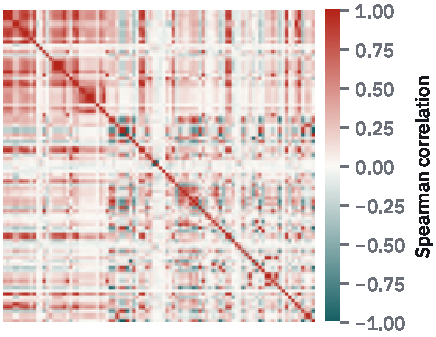
\includegraphics{heatmap.pdf}
  \caption{Spearman correlation matrix of the 94 ratios, in dataset column order. Blocks of near-duplicates (profitability, per-share values, growth, leverage, cash flow) motivate variable selection.}\label{fig:heatmap}
\end{figure}

% =====================================================================
\section{Methods and choices}
% =====================================================================

\subsection{Overview}
Figure~\ref{fig:pipeline} summarises the approach (``variable selection with decision-tree classification''). A LASSO logistic regression chooses a subset of ratios; a decision tree, grown on the raw values of those ratios, estimates the bankruptcy probability in each leaf; the Bayes rule~\eqref{eq:bayes} turns that probability into a decision.

\begin{figure}[htbp]\centering
  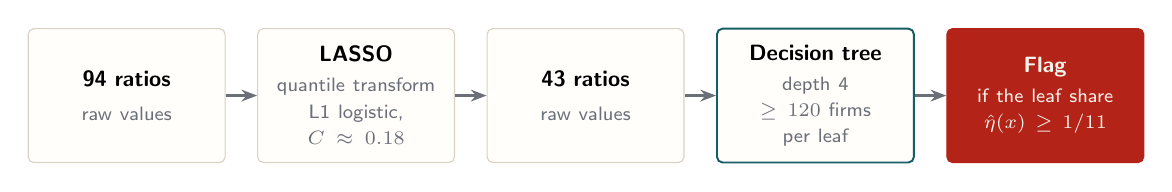
\begin{tikzpicture}[node distance=4mm, box/.style={draw=rule, fill=card, rounded corners=2pt, align=center, text width=22mm,
                      minimum height=17mm, inner sep=1.5mm, font=\sffamily\footnotesize}, arr/.style={-{Stealth[length=2mm]}, muted, line width=0.8pt}]
    \node[box] (a) {\textbf{94 ratios}\\[1mm]{\scriptsize\color{muted}raw values}};
    \node[box, right=of a] (b) {\textbf{LASSO}\\[1mm]{\scriptsize\color{muted}quantile transform\\L1 logistic, $C \approx 0.18$}};
    \node[box, right=of b] (c) {\textbf{43 ratios}\\[1mm]{\scriptsize\color{muted}raw values}};
    \node[box, right=of c, draw=model, line width=0.7pt] (d) {\textbf{Decision tree}\\[1mm]{\scriptsize\color{muted}depth 4\\$\ge 120$ firms per leaf}};
    \node[box, right=of d, fill=risk, draw=risk, text=paper] (e) {\textbf{Flag}\\[1mm]{\scriptsize if the leaf share\\$\hat\eta(x) \ge 1/11$}};
    \foreach \u/\v in {a/b, b/c, c/d, d/e} \draw[arr] (\u) -- (\v);
  \end{tikzpicture}
  \caption{The final pipeline. Everything left of the decision is refit inside every cross-validation fold.}\label{fig:pipeline}
\end{figure}

\subsection{Data split and validation protocol}
We hold out a stratified 20\,\% test set (1,364 firms, 44 bankrupt) with a fixed seed; the remaining 5,455 firms (176 bankrupt) form the training set. The test set is opened once, at the end, for the frozen final model and the baseline only (Lecture~2). All tuning and model comparisons use the \emph{same} stratified 5-fold cross-validation on the training set. Preprocessing and selection are part of scikit-learn pipelines~\cite{sklearn}, so in every fold the quantile transform, the LASSO and the tree are refit on four folds and scored on the fifth: no information leaks from the validation fold. Code~\ref{lst:metric} shows the metric used throughout.

\begin{lstlisting}[float=htbp, caption={The decision cost as a scikit-learn scorer (notebook, Section 3.1).}, label={lst:metric}]
def avg_cost(y_true, y_pred, c_fn=C_FN, c_fp=C_FP):
    return np.mean(c_fn * ((y_true == 1) & (y_pred == 0))
                   + c_fp * ((y_true == 0) & (y_pred == 1)))

cost_scorer = make_scorer(avg_cost, greater_is_better=False)
\end{lstlisting}

\subsection{Preprocessing}\label{sec:preproc}
The constant column is dropped. The 24 ratios with extreme values are \emph{not} capped: among the 4,816 training firms whose \texttt{Total Asset Growth Rate} exceeds 1, the value alone still ranks bankruptcies with an AUC of 0.72, so the extreme values carry signal. The two models need different treatments. The tree only uses the order of the values and receives the raw ratios. The LASSO is sensitive to scale, so it receives a rank-based quantile transform to a standard normal, fitted on the training folds only: it keeps the order of the values, removes the magnitude problem and puts all ratios on a common scale, which a fair L1 penalty requires.

\subsection{Variable selection: LASSO logistic regression}
For a binary outcome, the LASSO of Lecture~4 becomes an L1-penalised logistic regression with an unpenalised intercept:
\begin{equation}\label{eq:lasso}
  \min_{b_0,\,\beta}\; -\frac{1}{n}\sum_{i=1}^{n}\Big[y_i\log p_i + (1-y_i)\log(1-p_i)\Big] + \lambda\lVert\beta\rVert_1,
  \qquad p_i = \frac{1}{1+e^{-(b_0 + x_i^\top\beta)}} .
\end{equation}
The L1 penalty sets many coefficients exactly to zero; the corresponding ratios are dropped. In scikit-learn the penalty is set through $C = 1/(n\lambda)$. We prefer the LASSO to forward selection (Lecture~3.2) because a single parameter controls the number of variables, it copes with the redundant ratios, and one fit takes under a second, so it can be refit inside every fold; forward selection would need up to 94 fits per added variable, repeated in every fold. The intercept is kept unpenalised as in the course (\texttt{intercept\_scaling=100} makes \texttt{liblinear}'s intercept penalty negligible), and no class weights are used: the LASSO only chooses variables, and the costs enter at the decision stage.

\paragraph{Penalty} $C$ is chosen by 5-fold cross-validation on the training set, minimising the log-loss, a proper scoring rule and the classification counterpart of the validation MSE used in the course, over 13 values from $10^{-3}$ to $1$ (Code~\ref{lst:lasso}). The minimum, $C \approx 0.178$, keeps \textbf{43 of the 94 ratios}, with a CV log-loss of 0.0855 against 0.143 with no variable (Figure~\ref{fig:lasso}). The curve is flat: every $C$ from 0.056 (21 ratios) to 0.562 (59 ratios) is within one standard error of the minimum.

\begin{lstlisting}[float=htbp, caption={LASSO pipeline and choice of the penalty (notebook, Sections 2.1–2.2).}, label={lst:lasso}]
lasso = make_pipeline(QuantileTransformer(output_distribution="normal"),
                      LogisticRegression(l1_ratio=1, solver="liblinear",
                                         intercept_scaling=100, random_state=SEED))
cv = StratifiedKFold(n_splits=5, shuffle=True, random_state=SEED)
C_grid = np.logspace(-3, 0, 13)
lasso_cv = GridSearchCV(lasso, {"logisticregression__C": C_grid}, cv=cv,
                        scoring="neg_log_loss", n_jobs=-1).fit(X_train, y_train)
\end{lstlisting}

\begin{figure}[htbp]\centering
  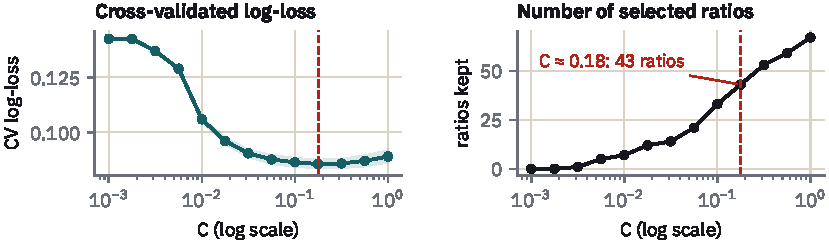
\includegraphics{lasso_path.pdf}
  \caption{Choice of the LASSO penalty. Left: cross-validated log-loss (mean $\pm$ 1 SE). Right: number of ratios kept when refit on the full training set. Dashed line: chosen $C \approx 0.18$.}\label{fig:lasso}
\end{figure}

\paragraph{What is selected, and how stable it is} The leading coefficients (Table~\ref{tab:coef}) cover leverage, profitability and liquidity, with intuitive signs: more debt raises the predicted risk, more profit and liquidity lower it. Following Lecture~4, we refit the whole procedure on 100 stratified bootstrap resamples of the training set (Figure~\ref{fig:stability}). Only 15 of the 43 selected ratios are kept in at least 80\,\% of the resamples, and some ratios left out are often selected, such as the R\&D expense rate (81\,\%): correlated ratios swap places. The selected set is a good predictive shortlist, not a list of causes.

\begin{table}[htbp]\centering\tablefont
  \caption{The eight largest LASSO coefficients at $C \approx 0.178$ (quantile-normal scale, so magnitudes are comparable).}\label{tab:coef}
  \begin{tabular}{lr@{\qquad}lr}
    \toprule
    Ratio & Coefficient & Ratio & Coefficient \\
    \midrule
    Total debt / total net worth & $+0.819$ & Quick ratio & $-0.320$ \\
    ROA(B) before interest & $-0.477$ & Working capital turnover & $+0.314$ \\
    Retained earnings / total assets & $-0.415$ & Persistent EPS (4 seasons) & $-0.311$ \\
    Interest-bearing debt interest rate & $+0.350$ & Borrowing dependency & $+0.308$ \\
    \bottomrule
  \end{tabular}
\end{table}

\begin{figure}[htbp]\centering
  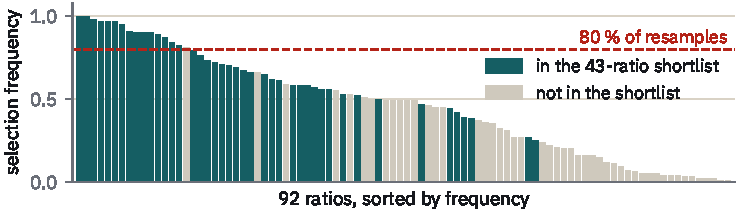
\includegraphics{stability.pdf}
  \caption{Selection stability: share of 100 bootstrap refits in which each ratio is selected (92 ratios selected at least once). Teal: in the 43-ratio shortlist; grey: not in it.}\label{fig:stability}
\end{figure}

\subsection{Decision tree and decision rule}
A classification tree (CART, Gini impurity $G(q) = 2q(1-q)$, Lecture~3) is grown on the raw values of the selected ratios. The share of bankrupt training firms in a leaf estimates $\hat\eta(x) = P(Y=1 \mid x)$ for every firm reaching it, and the firm is flagged when $\hat\eta(x) \ge 1/11$. The costs therefore enter through the \emph{threshold}, not through class weights: this keeps the leaves' reading as probabilities and lets us test other cost ratios without retraining. In code, the whole pipeline is wrapped in a \texttt{FixedThresholdClassifier}, so its predictions are directly the decisions (Code~\ref{lst:m2}).

\paragraph{Hyperparameters} We tune the maximum depth, $\{2,3,4,5,6,8,\text{no limit}\}$, and the minimum number of firms per leaf, $\{1,10,20,40,80,120,160,200\}$, on the decision cost. Large leaves are needed for the leaf shares to be reliable probabilities: with a 3.2\,\% bankruptcy rate, a leaf of 120 firms holds only about four bankruptcies. Figure~\ref{fig:validation} shows the effect. With leaves of one firm, the training cost falls to zero as the tree deepens while the CV cost climbs from 0.17 to 0.23: the tree memorises the training firms (Lecture~2). With at least 120 firms per leaf, the gap stays small and depth~4 is best (0.151).

\begin{lstlisting}[float=htbp, caption={Final pipeline M2 and its tuning (notebook, Sections 2.4 and 3.3).}, label={lst:m2}]
selector = SelectFromModel(lasso.set_params(logisticregression__C=best_C),
                           importance_getter="named_steps.logisticregression.coef_",
                           threshold=1e-5)  # keep the non-zero coefficients
pipe = FixedThresholdClassifier(
    Pipeline([("select", selector),
              ("tree", DecisionTreeClassifier(random_state=SEED))]),
    threshold=THRESHOLD)                    # flag when P(bankrupt | x) >= 1/11
tree_grid = {"max_depth": [2, 3, 4, 5, 6, 8, None],
             "min_samples_leaf": [1, 10, 20, 40, 80, 120, 160, 200]}
m2_grid = {"estimator__select__estimator__logisticregression__C": [best_C],
           **{f"estimator__tree__{k}": v for k, v in tree_grid.items()}}
m2 = GridSearchCV(pipe, m2_grid, cv=cv, scoring=cost_scorer, n_jobs=-1,
                  return_train_score=True).fit(X_train, y_train)
\end{lstlisting}

\begin{figure}[htbp]\centering
  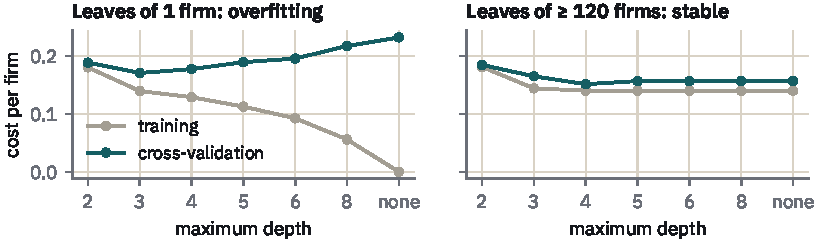
\includegraphics{validation.pdf}
  \caption{Validation curves of the final pipeline: training and cross-validated cost per firm against the maximum depth, for leaves of one firm (left) and of at least 120 firms (right).}\label{fig:validation}
\end{figure}

% =====================================================================
\section{Evaluation}
% =====================================================================

\subsection{Cross-validated model selection}
We compare four candidates on the same folds: \textbf{M0}, the baseline; \textbf{M1}, a tuned tree on all 94 ratios; \textbf{M2}, the LASSO selector with $C$ fixed at its Section~2.4 value, followed by a tuned tree; and \textbf{M3}, the same pipeline with $C$ tuned jointly with the tree over the seven grid values from 0.01 to 0.316. The selection rule was fixed before seeing these results: M2, the course protocol, is the reference, and an alternative replaces it only if its CV cost is lower by more than one standard error. Because all candidates share the folds, the comparison is \emph{paired}: for each fold $k$ we compute the gain $\Delta_k = \text{cost}_k(\text{M2}) - \text{cost}_k(\text{alternative})$ and its standard error $s_\Delta/\sqrt{5}$ (Code~\ref{lst:rule}).

\begin{table}[htbp]\centering\tablefont
  \caption{Cross-validated results (5 folds, training set). Paired gain of each alternative over M2: mean $\pm$ standard error, and number of folds in which it is cheaper than M2.}\label{tab:cv}
  \begin{tabular}{lcccccc}
    \toprule
    Candidate & CV cost & Depth & Leaf & $C$ & Ratios & Paired gain over M2 \\
    \midrule
    M0 Never flag & 0.323 & -- & -- & -- & 0 & $-0.171 \pm 0.009$ \ (0/5) \\
    M1 Tree, all ratios & 0.163 & 4 & 120 & -- & 94 & $-0.012 \pm 0.005$ \ (0/5) \\
    \textbf{M2 LASSO + tree} & \textbf{0.151} & 4 & 120 & 0.178 & 43 & reference \\
    M3 LASSO (joint $C$) + tree & 0.148 & 3 & 10 & 0.01 & 7 & $+0.003 \pm 0.007$ \ (3/5) \\
    \midrule
    \textcolor{bench}{M4 LASSO + random forest} & 0.136 & -- & 10 & 0.178 & 43 & $+0.015 \pm 0.007$ \ (5/5) \\
    \bottomrule
  \end{tabular}
\end{table}

\begin{lstlisting}[float=htbp, caption={Paired selection rule (notebook, Section 3.4).}, label={lst:rule}]
# per-fold gain of each candidate over M2 (> 0: cheaper than M2)
gains = fold_costs.rsub(fold_costs["M2 LASSO, C fixed"], axis=0)
rule = pd.DataFrame({"mean gain over M2": gains.mean(),
                     "paired SE": gains.std() / np.sqrt(5),
                     "folds cheaper than M2": (gains > 0).sum()})
rule["replaces M2"] = rule["mean gain over M2"] > rule["paired SE"]
\end{lstlisting}

Table~\ref{tab:cv} and Figure~\ref{fig:candidates} give the results. Every tree halves the cost of the baseline. \textbf{Variable selection helps}: M2 beats the tree on all 94 ratios by $0.012 \pm 0.005$ and is cheaper or tied on every fold. Joint tuning (M3) is not significantly better ($0.003 \pm 0.007$), although it shows that a 7-ratio selection works about as well. M2 is therefore the final model.

\paragraph{Benchmark: the price of interpretability} To measure what a single readable tree costs, we also cross-validated a random forest of 300 trees on the LASSO-selected ratios (M4), tuning its leaf size. It is a benchmark, not a candidate: the brief asks for a decision-tree classifier and our recommendation relies on reading the tree's rules, so M4 is never scored on the test set. It is about 10\,\% cheaper ($0.015 \pm 0.007$, cheaper on all five folds), because averaging 300 trees gives much finer probabilities than nine leaves.

\begin{figure}[htbp]\centering
  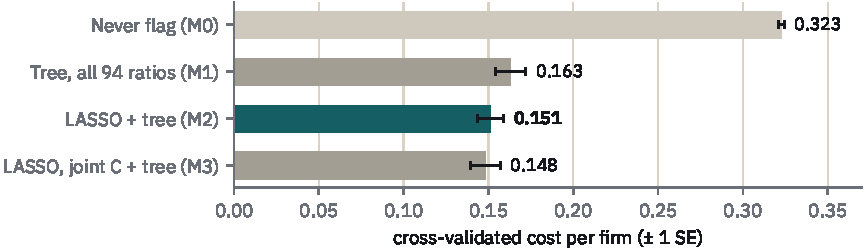
\includegraphics{candidates.pdf}
  \caption{Cross-validated cost per firm of the four candidates ($\pm$ 1 standard error across folds).}\label{fig:candidates}
\end{figure}

\subsection{The final model}
Refit on the full training set, the LASSO keeps 43 ratios and the tree, of depth~4, has \textbf{9 leaves and uses only 8 of them} (Figure~\ref{fig:tree}): the tree performs a second, finer selection.

\begin{figure}[htbp]\centering
  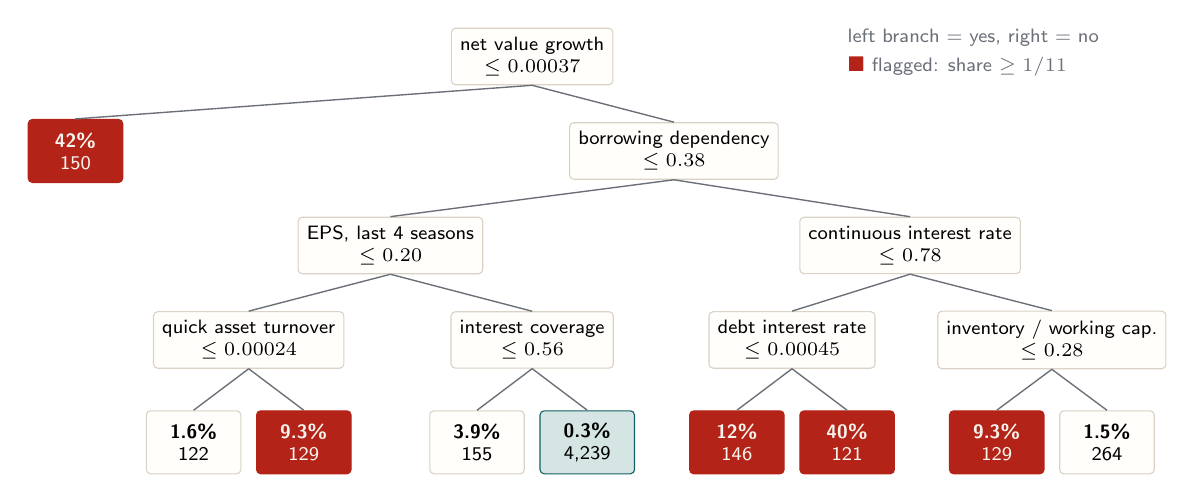
\begin{tikzpicture}[x=1mm, y=1mm, font=\sffamily\scriptsize,
      split/.style={draw=rule, fill=card, rounded corners=1.5pt, align=center, inner sep=1.1mm},
      leaf/.style={draw=rule, fill=card, rounded corners=1.5pt, align=center, inner sep=0.8mm, minimum width=12mm, minimum height=8mm},
      flag/.style={leaf, fill=risk, draw=risk, text=paper},
      e/.style={draw=muted, line width=0.5pt}]
    \node[split] (n0)  at (70,0)    {net value growth\\$\le 0.00037$};
    \node[flag]  (n1)  at (12,-12)  {\textbf{42\%}\\150};
    \node[split] (n2)  at (88,-12)  {borrowing dependency\\$\le 0.38$};
    \node[split] (n3)  at (52,-24)  {EPS, last 4 seasons\\$\le 0.20$};
    \node[split] (n10) at (118,-24) {continuous interest rate\\$\le 0.78$};
    \node[split] (n4)  at (34,-36)  {quick asset turnover\\$\le 0.00024$};
    \node[split] (n7)  at (70,-36)  {interest coverage\\$\le 0.56$};
    \node[split] (n11) at (103,-36) {debt interest rate\\$\le 0.00045$};
    \node[split] (n14) at (136,-36) {inventory / working cap.\\$\le 0.28$};
    \node[leaf]  (n5)  at (27,-49)  {\textbf{1.6\%}\\122};
    \node[flag]  (n6)  at (41,-49)  {\textbf{9.3\%}\\129};
    \node[leaf]  (n8)  at (63,-49)  {\textbf{3.9\%}\\155};
    \node[leaf, fill=modeltint, draw=model] (n9) at (77,-49) {\textbf{0.3\%}\\4,239};
    \node[flag]  (n12) at (96,-49)  {\textbf{12\%}\\146};
    \node[flag]  (n13) at (110,-49) {\textbf{40\%}\\121};
    \node[flag]  (n15) at (129,-49) {\textbf{9.3\%}\\129};
    \node[leaf]  (n16) at (143,-49) {\textbf{1.5\%}\\264};
    \foreach \a/\b in {n0/n1, n0/n2, n2/n3, n2/n10, n3/n4, n3/n7, n10/n11, n10/n14, n4/n5, n4/n6, n7/n8, n7/n9, n11/n12, n11/n13, n14/n15, n14/n16}
      \draw[e] (\a.south) -- (\b.north);
    \node[anchor=north west, align=left, text=muted, inner sep=0] at (110,3.5)
      {left branch = yes, right = no\\[0.8mm]{\color{risk}$\blacksquare$} flagged: share $\ge 1/11$};
  \end{tikzpicture}
  \caption{The final tree. Each leaf shows its share of bankrupt training firms and its number of firms; red leaves are flagged.}\label{fig:tree}
\end{figure}

\subsection{Test-set performance}
The frozen model and the baseline are scored once on the 1,364 test firms (Table~\ref{tab:test}, Code~\ref{lst:test}). The model \textbf{costs 0.179 per firm against 0.323}, a 45\,\% reduction. It catches 32 of the 44 bankruptcies (recall 73\,\%) at the price of 124 false alarms (precision 21\,\%): 156 firms are flagged, about one in nine. Its accuracy (90\,\%) is lower than the baseline's (97\,\%), which confirms that accuracy would have rewarded the useless rule.

\begin{table}[htbp]\centering\tablefont
  \caption{Test-set performance (1,364 firms, 44 bankrupt). Right: confusion matrix of the final model.}\label{tab:test}
  \begin{minipage}[c]{0.52\linewidth}\centering
    \begin{tabular}{lcc}
      \toprule
      & Final model & Never flag \\
      \midrule
      Average cost per firm & \textbf{0.179} & 0.323 \\
      Recall & 0.727 & 0.000 \\
      Precision & 0.205 & -- \\
      Accuracy & 0.900 & 0.968 \\
      Firms flagged & 156 & 0 \\
      \bottomrule
    \end{tabular}
  \end{minipage}\hfill
  \begin{minipage}[c]{0.44\linewidth}\centering
    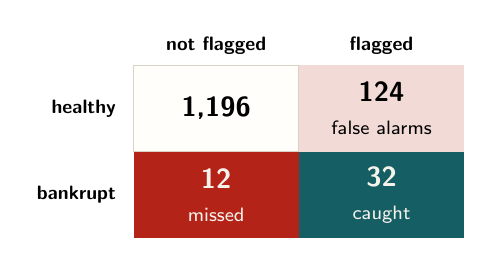
\begin{tikzpicture}[x=1mm, y=1mm, cell/.style={minimum width=21mm, minimum height=11mm, align=center, inner sep=0}]
      \node[font=\sffamily\scriptsize\bfseries] at (10.5,8) {not flagged};
      \node[font=\sffamily\scriptsize\bfseries] at (31.5,8) {flagged};
      \node[font=\sffamily\scriptsize\bfseries, anchor=east] at (-1,0) {healthy};
      \node[font=\sffamily\scriptsize\bfseries, anchor=east] at (-1,-11) {bankrupt};
      \node[cell, fill=card, draw=rule] at (10.5,0) {\textbf{1,196}};
      \node[cell, fill=risktint] at (31.5,0) {\textbf{124}\\{\scriptsize false alarms}};
      \node[cell, fill=risk, text=paper] at (10.5,-11) {\textbf{12}\\{\scriptsize missed}};
      \node[cell, fill=model, text=paper] at (31.5,-11) {\textbf{32}\\{\scriptsize caught}};
    \end{tikzpicture}
  \end{minipage}
\end{table}

\begin{lstlisting}[float=htbp, caption={Test predictions and bootstrap of the test costs (notebook, Sections 4.1–4.2).}, label={lst:test}]
y_pred = final_model.predict(X_test)        # decisions at the 1/11 threshold
y_base = np.zeros(len(y_test), dtype=int)   # "never flag"
boot = [resample(np.arange(len(y_test)), random_state=b) for b in range(1000)]
boot_costs = pd.DataFrame(
    [{"Final model": avg_cost(y_test.values[i], y_pred[i]),
      "Baseline": avg_cost(y_test.values[i], y_base[i])} for i in boot])
\end{lstlisting}

\paragraph{Uncertainty} With a loss bounded in $[0, C_{FN}]$ and $m = 1{,}364$ test firms, Lecture~2's Hoeffding bound gives a 95\,\% half-width of $C_{FN}\sqrt{\log(2/\alpha)/(2m)} = 0.37$, wider than the gap between the two rules: valid, but uninformative. We therefore use a 95\,\% percentile bootstrap over the test firms, with the predictions fixed and without stratification, so that the number of bankruptcies varies as in a new sample (Figure~\ref{fig:bootstrap}). The paired difference lies in $[-0.228, -0.065]$, entirely below zero: the model's advantage is not an artefact of this test set. The test cost is higher than the CV estimate (0.151), which nevertheless lies inside the model's interval; the gap is expected, since the test cost is noisy with only 44 bankruptcies and the CV cost of the chosen configuration, the best of 56, is slightly optimistic.

\begin{figure}[htbp]\centering
  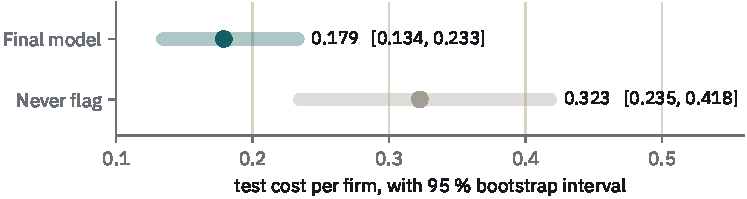
\includegraphics{bootstrap.pdf}
  \caption{Test cost per firm with 95\,\% bootstrap intervals (1,000 resamples of the test firms). Gain of the model over the baseline: $[0.065, 0.228]$ per firm.}\label{fig:bootstrap}
\end{figure}

\subsection{Sensitivity to the cost ratio}\label{sec:sensitivity}
The 10:1 ratio is an assumption. For a ratio $r = C_{FN}/C_{FP}$ the Bayes threshold becomes $1/(1+r)$; since the tree is not retrained, only the threshold changes (Table~\ref{tab:sens}). The model beats the baseline under every ratio, cutting its cost by 35\,\%, 45\,\% and 59\,\%. Each leaf is flagged once $r$ exceeds its \emph{switching ratio}
\begin{equation}\label{eq:switch}
  r^* = \frac{1-\hat\eta}{\hat\eta}, \qquad \text{since } \hat\eta \ge \frac{1}{1+r} \iff r \ge r^* .
\end{equation}
Figure~\ref{fig:switching} shows that the two riskiest leaves (42\,\% and 40\,\%) are flagged for any ratio above 1.5, while two leaves (9.3\,\%) switch at 9.75, just below our assumed ratio. No leaf switches between 9.75 and 24.8, which is why ratios 10 and 20 give identical decisions.

\begin{table}[htbp]\centering\tablefont
  \caption{Test-set results under three cost ratios (tree unchanged, threshold $1/(1+r)$).}\label{tab:sens}
  \begin{tabular}{ccccccc}
    \toprule
    Cost ratio $r$ & Threshold & Model cost & Baseline cost & Recall & Precision & Firms flagged \\
    \midrule
    5 & 0.167 & 0.106 & 0.161 & 0.545 & 0.353 & 68 \\
    \textbf{10} & \textbf{0.091} & \textbf{0.179} & \textbf{0.323} & \textbf{0.727} & \textbf{0.205} & \textbf{156} \\
    20 & 0.048 & 0.267 & 0.645 & 0.727 & 0.205 & 156 \\
    \bottomrule
  \end{tabular}
\end{table}

\begin{figure}[htbp]\centering
  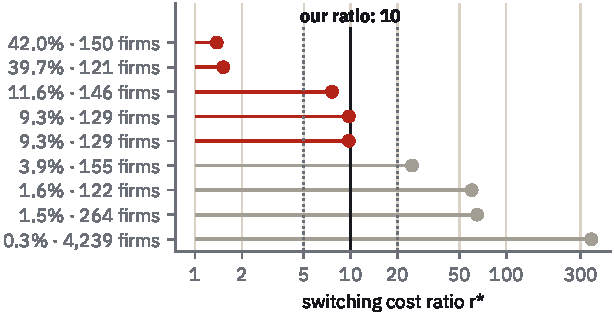
\includegraphics{switching.pdf}
  \caption{Switching cost ratio of each leaf (training share of bankrupt firms and number of firms). Red: flagged at our ratio of 10; dotted lines: ratios 5 and 20.}\label{fig:switching}
\end{figure}

% =====================================================================
\section{Evidence and recommendation}
% =====================================================================

\subsection{What the tree says}
Reading the flagged leaves of Figure~\ref{fig:tree}, the model raises an alarm in three situations: (i) the 2.7\,\% of firms with the weakest net value growth, of which 42\,\% went bankrupt; (ii) heavy reliance on borrowing combined with weak profitability, 40\,\% bankrupt when the debt is expensive and 12\,\% otherwise; (iii) two narrower pockets at 9.3\,\%, flagged only just. Conversely, firms with moderate borrowing, EPS above 0.20 and an interest coverage ratio above 0.56 hold 78\,\% of the training firms and a bankruptcy share of 0.3\,\%. These are predictive associations, not causal effects.

\subsection{Recommendation}
Following the decision-memo structure of Lecture~1:
\begin{enumerate}
  \item \textbf{Action and information.} Flag every firm whose leaf has a bankruptcy share of at least $1/11$, using 8 financial ratios read by a depth-4 tree.
  \item \textbf{Assumptions.} A missed bankruptcy costs ten false alarms, and the leaf shares of 5,455 training firms are taken as bankruptcy probabilities.
  \item \textbf{Comparison with the alternative.} On unseen firms the model costs 0.179 per firm against 0.323 without screening, catching 32 of 44 bankruptcies for 124 false alarms. A random forest would lower the cross-validated cost by about 10\,\%, but without the readable rules this recommendation relies on.
  \item \textbf{Conditions that would change the choice.} With a cost ratio below 9.75, two leaves would no longer be flagged, and below 7.6 a third; any ratio between 9.75 and 24.8 leaves the decisions unchanged.
\end{enumerate}

\subsection{Limitations}
\begin{itemize}
  \item \textbf{Stipulated costs.} The 10:1 ratio is an assumption, and two leaves depend on it being at least 9.75.
  \item \textbf{No time dimension.} Firms are pooled over 1999–2009 without a year, so the evaluation is a random split, not a forecast of future years; economic conditions may shift (Lecture~2).
  \item \textbf{Possibly repeated firms.} The rows may include several years of the same firm; a random split can then place one firm in both training and test, making the test cost optimistic. Without a firm identifier this cannot be checked.
  \item \textbf{Few bankruptcies.} With 176 bankruptcies in training and 44 in test, CV standard errors are about 0.008, the test interval is wide, and leaf shares rest on 2 to 63 bankruptcies. Nodes 6 and 15 are flagged with a share of 0.093, only 0.002 above the threshold, while that share's standard error is about $\sqrt{0.093 \times 0.907 / 129} \approx 0.026$.
  \item \textbf{No nested cross-validation.} M2 and M3 were compared on the folds used to tune them; the pre-registered rule limits but does not remove this optimism.
  \item \textbf{Unstable variable list.} Only 15 of the 43 LASSO ratios are robustly selected, and a 7-ratio selection works about as well.
  \item \textbf{Data quality.} Three of the eight ratios used by the tree contain extreme values that look like encoding artefacts; the order-based treatment limits, but may not remove, their impact.
\end{itemize}
Before deployment, the frozen procedure should be refit on all 6,819 firms and validated on more recent data.

% =====================================================================
\section{Reproducibility}
% =====================================================================
All results come from a single notebook, \texttt{src/bankruptcy\_prediction.ipynb}, executed top to bottom with fixed seeds (\texttt{SEED = 42}); it runs in about 4.5 minutes with Python 3.12 and the pinned versions of \texttt{requirements.txt} (scikit-learn 1.9.1, pandas 3.0.6). The notebook stops with an explicit message if scikit-learn is older than 1.8, because earlier versions silently replace the L1 penalty. A script, \texttt{slides/make\_figures.py}, exports the figures of this report from that same notebook.
\begin{lstlisting}[language=bash, aboveskip=4pt]
uv venv --python 3.12 && uv pip install -r requirements.txt
.venv/bin/jupyter nbconvert --to notebook --execute --inplace \
    src/bankruptcy_prediction.ipynb
\end{lstlisting}

% =====================================================================
\begin{thebibliography}{9}\footnotesize\setlength{\itemsep}{0.5pt}
\bibitem{uci} UCI Machine Learning Repository (2020). \emph{Taiwanese Bankruptcy Prediction}. doi:\href{https://doi.org/10.24432/C5004D}{10.24432/C5004D}.
\bibitem{liang} D.~Liang, C.-C.~Lu, C.-F.~Tsai and G.-A.~Shih (2016). Financial ratios and corporate governance indicators in bankruptcy prediction: a comprehensive study. \emph{European Journal of Operational Research}, 252(2), 561–572.
\bibitem{sklearn} F.~Pedregosa et al. (2011). Scikit-learn: machine learning in Python. \emph{Journal of Machine Learning Research}, 12, 2825–2830.
\bibitem{course} Augmented Decision, lecture decks 1–4: decision theory, statistical learning, decision trees, variable selection and regularization.
\end{thebibliography}

% =====================================================================
%  APPENDIX — LLM assistance (inputs in appendix/ are generated by build_appendix.py)
% =====================================================================
\clearpage
\appendix
\section{LLM assistance}

As the project brief requires, this appendix discloses how a large language model (LLM) helped prepare this work. It describes the tool and what it supported (A.1), the working protocol the authors imposed on it (A.2), the authors' decisions and modifications (A.3), every prompt the authors sent, verbatim (A.4), and the full content of the protocol and discussion files (A.5).

\subsection{Tool and scope}
We used \textbf{Claude Opus 5.5} (Anthropic) through \textbf{Claude Code}, its coding assistant integrated in Visual Studio Code, during a single working session on 22 October 2026. The LLM worked inside the project folder: it read the files (including the lecture decks and the brief), ran code in the project's Python environment, and wrote files. Every part of this report was prepared with the LLM; Table~\ref{tab:llm} identifies what it supported and what the authors did.

\begin{table}[htbp]\centering\tablefont
  \caption{Parts of the work supported by the LLM.}\label{tab:llm}
  \begin{tabularx}{\linewidth}{>{\raggedright\arraybackslash}p{38mm}XX}
    \toprule
    Part & Role of the LLM & Role of the authors \\
    \midrule
    The notebook, source of every number, table and figure of this report & Wrote the code and markdown cells following the approved plans, ran the notebook, exported the figures & Wrote the rules, reviewed and edited every plan, chose between the options, reviewed code and recaps, edited cells \\
    Report, Sections 1–5 (text, tables, figures, code snapshots) & Drafted the whole report from the notebook outputs & Specified the content (project brief), reviewed \\
    Appendix A & Assembled from \texttt{INSTRUCTIONS.md}, the AgentDiscussion files and the session transcript & Specified its content \\
    Slide deck, README, repository & Built on request & Specified the constraints, reviewed \\
    \bottomrule
  \end{tabularx}
\end{table}

\subsection{Working protocol}
Before starting, the authors wrote \texttt{INSTRUCTIONS.md} (reproduced in A.5). It fixes three things: the deliverable (one notebook implementing the four steps of this report), \textbf{simplicity rules} for the code (one task per cell, minimal code, a comment at the top of every cell, each step building on the previous one, every assumption or decision stated in a short markdown cell, a coherent markdown structure), and a \textbf{step-by-step workflow} instead of a one-shot project (Figure~\ref{fig:loop}).

\begin{figure}[htbp]\centering
  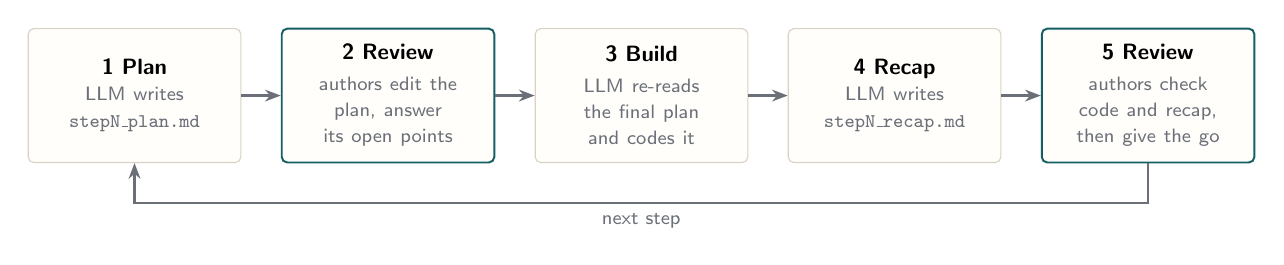
\begin{tikzpicture}[node distance=5mm, box/.style={draw=rule, fill=card, rounded corners=2pt, align=center, text width=24mm,
                      minimum height=17mm, inner sep=1.5mm, font=\sffamily\footnotesize},
                      human/.style={box, draw=model, line width=0.7pt}, arr/.style={-{Stealth[length=2mm]}, muted, line width=0.8pt}]
    \node[box] (p) {\textbf{1 Plan}\\[0.5mm]{\scriptsize\color{muted}LLM writes\\\texttt{stepN\_plan.md}}};
    \node[human, right=of p] (e) {\textbf{2 Review}\\[0.5mm]{\scriptsize\color{muted}authors edit the plan, answer its open points}};
    \node[box, right=of e] (b) {\textbf{3 Build}\\[0.5mm]{\scriptsize\color{muted}LLM re-reads the final plan and codes it}};
    \node[box, right=of b] (r) {\textbf{4 Recap}\\[0.5mm]{\scriptsize\color{muted}LLM writes\\\texttt{stepN\_recap.md}}};
    \node[human, right=of r] (v) {\textbf{5 Review}\\[0.5mm]{\scriptsize\color{muted}authors check code and recap, then give the go}};
    \foreach \u/\v in {p/e, e/b, b/r, r/v} \draw[arr] (\u) -- (\v);
    \draw[arr] (v.south) -- ++(0,-5mm) -| node[pos=0.25, below, font=\sffamily\scriptsize, text=muted] {next step} (p.south);
  \end{tikzpicture}
  \caption{The plan–recap loop of \texttt{INSTRUCTIONS.md}, run once per step. Teal: the authors; grey: the LLM.}\label{fig:loop}
\end{figure}

The written trace of this loop is the \texttt{AgentDiscussion} folder, with one sub-folder per step. A \textbf{plan} (\texttt{stepN\_plan.md}) was written at the start of each step: the LLM's thoughts, assumptions and rationale, the decisions it would record in the notebook, the planned cells, a preview from training-set checks, and a closing list of \emph{points for the authors to confirm or change}. The authors reviewed it, edited it directly when they disagreed (for instance, Step~1, \S5), and answered the open points in the conversation; their decisions were then recorded in the plan as ``decided''. The LLM re-read the plan in its final state before coding. A \textbf{recap} (\texttt{stepN\_recap.md}) was written after coding: what was built, the key results, every difference from the plan, and what carries over to the next step. The next step started only after the authors had reviewed the code and the recap. After Step~4, the authors added a \textbf{final review}: they asked for a critical assessment without any modification, then decided on each proposed fix one at a time, after asking what it would bring.

\subsection{Authors' decisions and modifications}
Table~\ref{tab:decisions} summarises how the authors steered the work; the numbers refer to the prompts of A.4.

\begin{table}[htbp]\centering\tablefont
  \caption{Main decisions and modifications made by the authors.}\label{tab:decisions}
  \begin{tabularx}{\linewidth}{>{\raggedright\arraybackslash}p{27mm}X}
    \toprule
    Phase (prompts) & Decisions and modifications \\
    \midrule
    Setup (1–2) & Let the LLM create the Python environment; required the notebook to be saved with its outputs; approved the file naming; quality not to be sacrificed to the deadline. \\
    Step 1 (3–5) & Edited the plan to run the exploratory analysis on the full dataset; kept the 10:1 costs and the 20\,\% test set; asked for a correlation matrix (accepting Spearman over Pearson) and for proper mathematical rendering. \\
    Step 2 (6–10) & Asked to compare the course rule for the LASSO penalty with tuning it jointly with the tree, under a one-standard-error rule; asked for an explanation of the stability plot, which led to a legend and an 80\,\% line; added their own explanation cell, an imports glossary and a plotting style to the notebook. \\
    Step 3 (11–12) & Followed the recommendations: costs through the threshold, the tuning grid, and the agreed selection rule without a tie-breaker. \\
    Step 4 (13–15) & Restricted the test set to the final model and the baseline; asked for explanations of the bootstrap and of the switching ratios before approving. \\
    Final review (16–33) & Asked for a critical review without modification; applied, after discussing each one, the version check, the repeated-firms limitation, the paired comparison and the leaf-noise limitation; removed every claim whose numbers the notebook did not reproduce, for simplicity; kept the single tree and added the random-forest benchmark. \\
    Organisation & Moved the notebook to \texttt{src/}, sorted \texttt{AgentDiscussion} into one folder per step, and removed the log of the final review. \\
    Deliverables (34–43) & Requested the README, the push to GitHub with the course material excluded, the slide deck (Arial version kept), this report and this appendix. \\
    \bottomrule
  \end{tabularx}
\end{table}

\subsection{Prompt log}
The 43 prompts sent by the authors during the session, verbatim, as typed. Context lines added automatically by the editor (such as the name of the file open in the IDE) are omitted; times are in UTC. The LLM's answers took the form of the plan and recap files of A.5, of the work itself, and of explanations given in the conversation.

\medskip
% Generated by build_appendix.py: the authors' prompts, verbatim
\promptentry{1}{Setup}{2026-10-22 08:34 UTC}{Hey Claude, take a look at the project and the INSTRUCTIONS.md file and confirm that you understand how we will proceed.\newline If any questions, ask them}
\promptentry{2}{Setup}{2026-10-22 08:40 UTC}{1. No environment for now, you can build one.\newline 2. Yes\newline 3. perfect\newline 4. Indeed but let's not sacrifice quality}
\promptentry{3}{Step 1}{2026-10-22 08:51 UTC}{Go}
\promptentry{4}{Step 1}{2026-10-22 09:04 UTC}{Can we add a correlation matrix to the EDA ?}
\promptentry{5}{Step 1}{2026-10-22 09:09 UTC}{One last detail, the markdown rendering for mathematical expression in 1.1 are not great (example : C\_FN etc), do you think you could apply actual adapted mathematical markdown for these expressions'}
\promptentry{6}{Step 2}{2026-10-22 09:11 UTC}{Excellent, let's move on to part 2.}
\promptentry{7}{Step 2}{2026-10-22 09:30 UTC}{Would it be sound to do as in the course (lowest cross-validated log-loss) and compare it with the method of tuning it together with the tree in step 3 ?}
\promptentry{8}{Step 2}{2026-10-22 09:31 UTC}{Go}
\promptentry{9}{Step 2}{2026-10-22 09:44 UTC}{Can you explain the bootstrap selection frequency plot ? Im not sure to understand it. \newline Explain the two colors}
\promptentry{10}{Step 2}{2026-10-22 09:54 UTC}{Yes make that change.}
\promptentry{11}{Step 3}{2026-10-22 09:57 UTC}{Excellent, let's move on to the step 3 plan.}
\promptentry{12}{Step 3}{2026-10-22 10:05 UTC}{Go, let's follow your recommendation}
\promptentry{13}{Step 4}{2026-10-22 11:21 UTC}{Let's move on to the step 4 plan}
\promptentry{14}{Step 4}{2026-10-22 11:28 UTC}{1. Only the final model and the baseline\newline 2. explain what you mean \newline 3. explain what you mean}
\promptentry{15}{Step 4}{2026-10-22 11:30 UTC}{Go}
\promptentry{16}{Final review}{2026-10-22 12:04 UTC}{Great, now I want you to take a step back, review the full codebase, then the notebook. Do not modify a single thing, I just want you to look at it, be critical, and come up with a fair judgement of what we have done. Are there an pothholes, is it solid and rigorous ? \newline Evaluate and come back here in the discussion with a report. \newline Be concize and straight to the point. \newline If any issues, suggest improvements.}
\promptentry{17}{Final review}{2026-10-22 12:18 UTC}{For point 3, is the absent evidence important or can we simply get rid of it ?}
\promptentry{18}{Final review}{2026-10-22 12:19 UTC}{As you know, our goal is to make the work the simplest possible, therefore, get rid of everything you can get rid of without destroying the reasoning.}
\promptentry{19}{Final review}{2026-10-22 12:23 UTC}{What could we expect from fixing number 2 ?}
\promptentry{20}{Final review}{2026-10-22 12:24 UTC}{Go for it}
\promptentry{21}{Final review}{2026-10-22 12:24 UTC}{what would fixing \#1 look like ?}
\promptentry{22}{Final review}{2026-10-22 12:25 UTC}{Go for it}
\promptentry{23}{Final review}{2026-10-22 12:31 UTC}{What would we gain from fixing \#4 ?}
\promptentry{24}{Final review}{2026-10-22 12:40 UTC}{Let's fix it.}
\promptentry{25}{Final review}{2026-10-22 12:50 UTC}{Explain what we gain from fixing \#5 ?}
\promptentry{26}{Final review}{2026-10-22 12:56 UTC}{Can we fix this while staying as simple as we want to ?}
\promptentry{27}{Final review}{2026-10-22 12:56 UTC}{Go}
\promptentry{28}{Final review}{2026-10-22 12:59 UTC}{Excellent, now there is one issue I am concerned with, the perfomance of the model. What can we do to improve it ?}
\promptentry{29}{Final review}{2026-10-22 13:03 UTC}{Ok let's [Request interrupted by user]}
\promptentry{30}{Final review}{2026-10-22 13:03 UTC}{Let's go with A.}
\promptentry{31}{Final review}{2026-10-22 13:12 UTC}{How many lines of code/\allowbreak{}comments/Markdown are there in the full notebook ? \newline Make a short summary table.}
\promptentry{32}{Final review}{2026-10-22 13:17 UTC}{What are the results of the random forest model ? compare them to the tree}
\promptentry{33}{Final review}{2026-10-22 13:29 UTC}{Do we now have the final version of the notebook ?}
\promptentry{34}{Repository}{2026-10-22 13:38 UTC}{Yes let's now build the final README for this project, make it professional and visually beautiful. Do not make it too long.}
\promptentry{35}{Repository}{2026-10-22 13:40 UTC}{are these also clickable links ?\par ![Python](https:/\allowbreak{}/\allowbreak{}img.shields.io/\allowbreak{}badge/\allowbreak{}Python-3.12-3776AB?\allowbreak{}logo=\allowbreak{}python\&logoColor=white)\newline ![scikit-learn](https:/\allowbreak{}/\allowbreak{}img.shields.io/\allowbreak{}badge/\allowbreak{}scikit-{}-learn-1.9-F7931E?\allowbreak{}logo=\allowbreak{}scikitlearn\&logoColor=white)\newline ![pandas](https:/\allowbreak{}/\allowbreak{}img.shields.io/\allowbreak{}badge/\allowbreak{}pandas-3.0-150458?\allowbreak{}logo=\allowbreak{}pandas\&logoColor=white)\newline ![Data](https:/\allowbreak{}/\allowbreak{}img.shields.io/\allowbreak{}badge/\allowbreak{}data-UCI\%20·\%20CC\%20BY\%204.0-lightgrey)}
\promptentry{36}{Repository}{2026-10-22 13:41 UTC}{YES}
\promptentry{37}{Repository}{2026-10-22 13:43 UTC}{Let's push the folder to the following repo : git remote add origin https:/\allowbreak{}/\allowbreak{}github.com/\allowbreak{}yassineerraji/\allowbreak{}Augmented-Decision-Final-Project.git\par Before that, let's create a .gitignore to avoid tracking DS\_Store and .venv.}
\promptentry{38}{Slide deck}{2026-10-22 13:56 UTC}{Great, now we want to build a slide deck to present for our final presentation. \newline For context, it should not exceed 15 minutes and should include the essentials of our project.\par The names are Yassine ERRAJI, William PELTIER, Ben DAESH, Simon AMAR\newline We want the slides to be very clean and professional yet very original and not look like the main claude templates. It should stand out.\par It should be built in LaTeX and compiled in pdf, obviously following the classic landscape slide deck format.\par Include the very main formulas that we build the project on top of (avoid the too complex ones that do not appear in the lecture decks). \newline Include the most relevant visuals that we obtained from the notebook (make sure that its format is adapted to the slide deck).\newline Also include schemas or graphs that you create on your own if you believe it would help present better and help people understand better our project.\par One Important element, slides must be readable and not too dense, therefore, we would rather have more slides that are more readable and less content heavy that fewer dense ones.\par Let's do this inside of a slides folder at the root of the repo.}
\promptentry{39}{Slide deck}{2026-10-22 15:36 UTC}{In the slide 25/28, in the head of the plot, the text is not well displayed (our ratio: 10), fix it.}
\promptentry{40}{Report}{2026-10-22 15:43 UTC}{Okay great now we want to build a properly compiled PDF report containing:\newline •Methods and choices. Explain your approach. Motivate the model, preprocessing, and\newline hyperparameters, e.g., tree depth, leaf size, or regularization penalty.\newline •Evaluation. Compare with a baseline. Tune by validation or cross-validation, fitting\newline preprocessing and selection within each training split. Report final test performance.\newline •Evidence and recommendation. Include readable code snapshots, labeled plots, and\newline result tables that justify your final model or variable set, recommendation, and limitations.\par Build it in a folder called report}
\promptentry{41}{Slide deck}{2026-10-22 15:57 UTC}{Now I want you to reproduce another exactly same version of the slide deck we have but this time using the Arial font.}
\promptentry{42}{Slide deck}{2026-10-22 16:06 UTC}{Okay excellent, let's delete the previous version and keep the arial one as the main.}
\promptentry{43}{Appendix}{2026-10-22 16:37 UTC}{Great, we want to add an appendix to the report about LLM Assistance (take a look at the ProjectRequirements.pdf).\newline In that section we must explain exactly the procedure of the INSTRUCTIONS.md and AgentDiscussion folder. \newline Detail the workflow of plan and recap, my modifications and instructions etc..\par If possible, include the content of the files in a nice rendering.}


\subsection{Protocol and discussion files}
The files below are reproduced in full, rendered from Markdown, as they stand at the end of the project. Paths written inside them reflect the folder layout at the time (the notebook was later moved from \texttt{notebooks/} to \texttt{src/}).

% Generated by build_appendix.py: INSTRUCTIONS.md and AgentDiscussion files rendered with pandoc
\begin{mdfile}{INSTRUCTIONS.md}{Working rules and workflow, written by the authors}
\mdh{1}{We are working on the Taiwanese Bankruptcy Prediction}

\begin{itemize}
\tightlist
\item
  (\url{https://archive.ics.uci.edu/dataset/572/taiwanese+bankruptcy+prediction}), UCI Machine Learning Repository. Collected from the Taiwan Economic Journal, 1999--2009.
\end{itemize}

\mdh{2}{Our goal is to build a 4-step project that goes as follows:}

\begin{enumerate}
\def\labelenumi{\arabic{enumi}.}
\tightlist
\item
  Problem Formulation \& Exploratory Data Analysis
\item
  Variable Selection
\item
  Model Selection and Decision Tree Tuning
\item
  Evaluation of the final model
\end{enumerate}

Our end-deliverable is one notebook file (ipynb), containing the code that implements the 4 steps.

\textbf{IMPORTANT}: WE MUST CODE IN THE MOST SIMPLE WAY POSSIBLE. WHAT IS MEANT BY SIMPLE IS:

\begin{itemize}
\tightlist
\item
  A python cell only does one task at a time.
\item
  We always privilege code minimality, what can be done in two lines of codes must be done in no more than two lines, always.
\item
  We always privilege simplicity and correctness over complexity and long code that is hard to visually understand.
\item
  We always include comments in the beginning of a Python cell to explain what is being done.
\item
  All the steps we code must build on top of the previous ones.
\item
  When doing assumptions, or making decisions, they must never be done silently and appear in the form of concise markdowns cells.
\item
  Markdown cells must follow a clean and coherent structure all the way through the notebook.
\end{itemize}

\mdh{2}{In the context folder you will find two elements:}

\begin{enumerate}
\def\labelenumi{\arabic{enumi}.}
\tightlist
\item
  The lecture decks of the course that will serve as great context to scope well the work we are doing.
\item
  The official instruction file for the project, provided by our teacher. Feel free to read it to have context on the final submission but don\textquotesingle t pay too much attention to it for now as we are only working on the code in a notebook for now. Also, don\textquotesingle t pay attention to the LLM disclosure element, I will take care of it when writing the report file.
\end{enumerate}

\mdh{2}{The workflow will be as follows:}

We will be working step by step and not one-shot the full project.

\begin{enumerate}
\def\labelenumi{\arabic{enumi}.}
\tightlist
\item
  You will explain very concisely your thoughts, assumptions and rationale in a folder called AgentDiscussion, where you will add a new markdown file at the beginning of each of the 4 steps of the project.
\item
  I will review in details the markdown files and either leave them as is or bring modification to them.
\item
  You will check the last state of the markdown cell and build according to it.
\item
  After you end coding, write a recap markdown file in the same AgentDiscussion folder and wait for me to review the code and the markdown file before signaling that we can proceed with the next step of the project.
\end{enumerate}
\end{mdfile}

\begin{mdfile}{AgentDiscussion/\allowbreak{}step1/\allowbreak{}step1\_plan.md}{Step 1 plan: written by the LLM, reviewed and edited by the authors}
\mdh{1}{Step 1 --- Problem Formulation \& EDA (plan)}

\mdh{2}{1. Problem formulation}

{\def\LTcaptype{none} % do not increment counter
\begin{tabularx}{\linewidth}{@{}l>{\raggedright\arraybackslash}X@{}}
\toprule\noalign{}
Element & Proposal \\
\midrule\noalign{}
\textbf{Target} & \texttt{Bankrupt?} (1 = the firm went bankrupt under Taiwan Stock Exchange rules, 0 = it did not) \\
\textbf{Inputs} & 95 financial ratios, assumed to be known \emph{before} the outcome (so no leakage) \\
\textbf{Decision supported} & A credit analyst decides whether to \textbf{flag} a firm as high-risk (deny or reprice credit, start a closer review) or \textbf{not flag} it \\
\textbf{Actions} & a = 1 flag, a = 0 do not flag \\
\bottomrule
\end{tabularx}
}

\textbf{Loss table (Lecture 1)}. This is an assumption, not an estimate:

{\def\LTcaptype{none} % do not increment counter
\begin{tabularx}{\linewidth}{@{}l>{\raggedright\arraybackslash}X>{\raggedright\arraybackslash}X@{}}
\toprule\noalign{}
& Healthy (Y = 0) & Bankrupt (Y = 1) \\
\midrule\noalign{}
Not flag (a = 0) & 0 & \textbf{C\_FN = 10} (credit loss) \\
Flag (a = 1) & \textbf{C\_FP = 1} (unnecessary review, lost client) & 0 \\
\bottomrule
\end{tabularx}
}

\begin{itemize}
\tightlist
\item
  \textbf{Bayes decision rule:} flag a firm when P(bankrupt \textbar{} x) ≥ C\_FP / (C\_FP + C\_FN) = \textbf{1/11 ≈ 0.09}.
\item
  \textbf{Primary metric:} average misclassification cost per firm, (10·FN + 1·FP) / n. This is the empirical risk under the loss table, so lower is better.
\item
  \textbf{Secondary metrics:} the confusion matrix, recall (share of bankruptcies caught) and precision (share of flags that are real bankruptcies).
\item
  \textbf{Why not accuracy:} only 3.2\% of firms are bankrupt, so "never flag" already reaches 96.8\% accuracy.
\item
  \textbf{Reference baseline:} "never flag" (the majority class) costs about 10 × 0.032 ≈ \textbf{0.32 per firm}. Every model has to beat this.
\item
  \textbf{Sensitivity:} in Step 4 we will re-run the evaluation with cost ratios of 5 and 20, because 10 is a stated assumption.
\end{itemize}

\mdh{2}{2. Assumptions and decisions (each one becomes a short markdown cell)}

\begin{enumerate}
\def\labelenumi{\arabic{enumi}.}
\tightlist
\item
  \textbf{The data has no firm ID and no year, so firms are treated as independent draws.} A time-based split is impossible, so we use a random stratified split. This becomes a stated limitation in Step 4.
\item
  \textbf{Drop \texttt{Net\ Income\ Flag}.} It has the same value in every row, so it carries no information.
\item
  \textbf{Hold out a stratified 80/20 train/test split right after loading} (\texttt{random\_state\ =\ 42}). That gives a test set of about 1,364 firms, about 44 of them bankrupt. The test set stays locked until Step 4.
\item
  \textbf{Run the EDA on the training set only}, so that no later decision uses test information (Lecture 2: "condition on every choice made using training data").
\item
  \textbf{Leave the raw values unchanged in Step 1.} 24 columns mix values in {[}0, 1{]} with values between about 6e5 and 1e10. Some columns have only a few such values; for others it is most rows (e.g. \texttt{Total\ Asset\ Growth\ Rate}: 6,017 of 6,819). These values look like an encoding artifact. A decision tree only depends on the order of the values, so it is unaffected. A linear selector (LASSO) is affected, so its treatment is decided in Step 2 and fitted inside the cross-validation folds.
\end{enumerate}

\mdh{2}{3. Notebook structure (applies to the whole notebook)}

\begin{Verbatim}[breaklines, fontsize=\footnotesize]
# Taiwanese Bankruptcy Prediction        ← title, dataset citation, 4-step overview
## 0. Setup                              ← imports, constants (SEED, C_FN, C_FP, THRESHOLD)
## 1. Problem Formulation & EDA
### 1.1 Problem formulation
### 1.2 Data loading and integrity checks
### 1.3 Train/test split
### 1.4 Exploratory analysis (training set)
### 1.5 Step 1 takeaways
## 2. Variable Selection                 ← same sub-structure, defined in Step 2's plan
...
\end{Verbatim}

\begin{itemize}
\tightlist
\item
  Decisions and assumptions are blockquotes: \texttt{\textgreater{}\ **Decision:**\ …} or \texttt{\textgreater{}\ **Assumption:**\ …}.
\item
  Findings are one-line \texttt{**Observation:**\ …} cells placed after the output they describe.
\item
  Dataset citation: UCI ML Repository, \emph{Taiwanese Bankruptcy Prediction}, DOI 10.24432/C5004D. Original study: Liang et al. (2016), \emph{European Journal of Operational Research} 252(2).
\end{itemize}

\mdh{2}{4. Planned code cells (one task each)}

{\def\LTcaptype{none} % do not increment counter
\begin{tabularx}{\linewidth}{@{}l>{\raggedright\arraybackslash}X@{}}
\toprule\noalign{}
\# & Cell \\
\midrule\noalign{}
1 & Imports \\
2 & Constants: \texttt{SEED}, \texttt{C\_FN}, \texttt{C\_FP}, \texttt{THRESHOLD} \\
3 & Load the CSV and strip the leading spaces from column names \\
4 & Shape and first rows \\
5 & Missing values and duplicate rows \\
6 & Target counts and proportions \\
7 & Bar plot of the target \\
8 & Find the constant columns, then drop them \\
9 & Split into X and y, then stratified train/test split \\
10 & Check the bankrupt rate in train and test \\
11 & Scale check: columns with values \textgreater{} 1 (count per column) \\
12 & Redundancy: number of feature pairs with \textbar r\textbar{} \textgreater{} 0.95, plus the top pairs \\
13 & Univariate signal: ROC-AUC of each feature alone, top 10 \\
14 & Boxplots of the 4 strongest features by class \\
\bottomrule
\end{tabularx}
}

What I expect to find, from a first look: 23 feature pairs with \textbar r\textbar{} \textgreater{} 0.95, several of them exact duplicates (r = 1.00). Profitability ratios (EPS, ROA, net income / assets) separate the classes best on their own, with AUC around 0.86--0.89. Both points motivate Step 2.

\mdh{2}{5. Points for you to confirm or change}

\begin{itemize}
\tightlist
\item
  \textbf{Cost ratio C\_FN : C\_FP = 10 : 1.} Alternatives: about 30 : 1, which roughly corresponds to balancing the two classes, or a non-cost metric such as F1 or recall at a fixed precision.
\item
  \textbf{Test size of 20\%.} Moving to 25\% gives about 55 bankrupt firms in the test set instead of 44.
\item
  **EDA on the full dataset.
\end{itemize}

\mdh{2}{Environment}

The project has a \texttt{.venv} created with \texttt{uv} (Python 3.12), and the dependencies are pinned in \texttt{requirements.txt}. The notebook will be saved with its outputs, at \texttt{notebooks/bankruptcy\_prediction.ipynb}.
\end{mdfile}

\begin{mdfile}{AgentDiscussion/\allowbreak{}step1/\allowbreak{}step1\_recap.md}{Step 1 recap: written by the LLM, reviewed by the authors}
\mdh{1}{Step 1 --- Problem Formulation \& EDA (recap)}

\textbf{Notebook:} \texttt{notebooks/bankruptcy\_prediction.ipynb}, sections 0 and 1. It runs end to end on the \texttt{.venv} kernel and is saved with its outputs.

\mdh{2}{What was built}

{\def\LTcaptype{none} % do not increment counter
\begin{tabularx}{\linewidth}{@{}l>{\raggedright\arraybackslash}X@{}}
\toprule\noalign{}
Section & Content \\
\midrule\noalign{}
Title & Short introduction, dataset citation, outline of the 4 steps \\
0. Setup & Imports; constants \texttt{SEED\ =\ 42}, \texttt{C\_FN\ =\ 10}, \texttt{C\_FP\ =\ 1}, \texttt{THRESHOLD\ =\ 1/11} \\
1.1 Problem formulation & Target, inputs, decision, loss table, Bayes rule, metric, baseline, plus 2 assumption cells (costs; no leakage and independent firms) \\
1.2 Loading and integrity & Load and clean column names; shape; missing values and duplicates; class counts and bar plot; drop the constant column; separate X and y \\
1.3 Exploratory analysis & Values above 1; Spearman correlation matrix (heatmap) and correlated pairs; AUC of each feature alone; boxplots of the top 4 features \\
1.4 Train/test split & Stratified 80/20 split and a check of both sets \\
1.5 Takeaways & 5 bullets that summarise the step \\
\bottomrule
\end{tabularx}
}

There are 18 code cells and 7 blockquote cells (decisions and assumptions), plus one \texttt{**Observation:**} line after each output that needs interpreting.

\mdh{2}{Key results}

\begin{itemize}
\tightlist
\item
  \textbf{Data quality:} 6,819 firms, no missing values, no duplicate rows. \texttt{Net\ Income\ Flag} has the same value everywhere and is dropped, which leaves \textbf{94 features}.
\item
  \textbf{Class imbalance:} 220 bankrupt firms (3.2\%). The "never flag" baseline costs about \textbf{0.32 per firm}.
\item
  \textbf{Extreme values:} 24 features mix values in {[}0, 1{]} with values between 6e5 and 1e10, with nothing in between. A few firms are affected in some features; 6,017 firms are affected in \texttt{Total\ Asset\ Growth\ Rate}.
\item
  \textbf{Redundancy:} 50 pairs of features have Spearman \textbar \ensuremath{\rho}\textbar{} \textgreater{} 0.95. These pairs involve 47 of the 94 features, and 13 of the pairs have \textbar \ensuremath{\rho}\textbar{} \textgreater{} 0.999. The heatmap shows blocks of related ratios: profitability, per-share values, growth, leverage and cash flow.
\item
  \textbf{Signal:} the strongest single predictors are profitability ratios (EPS, net income / assets, ROA), with AUC between 0.86 and 0.89. Bankrupt firms clearly score lower, but the two classes still overlap.
\item
  \textbf{Split:} 5,455 firms for training (176 bankrupt) and 1,364 for testing (44 bankrupt).
\end{itemize}

\mdh{2}{Differences from the plan}

\begin{enumerate}
\def\labelenumi{\arabic{enumi}.}
\tightlist
\item
  \textbf{Exploration on the full dataset.} I followed your edit in section 5 of the plan. Two places in the plan still say "training set only": §2 item 4 and the §3 outline. I treated your section 5 edit as the decision.
\item
  \textbf{Section order is now 1.3 EDA \ensuremath{\rightarrow} 1.4 split} (the plan had split \ensuremath{\rightarrow} EDA). Since the exploration uses the full data, splitting before it would serve no purpose, and the notebook reads more naturally this way. Tell me if you want the original order back.
\item
  \textbf{The "find constant columns, then drop them" step is two cells}, with the decision cell in between. This follows the "one task per cell" rule.
\item
  \textbf{Separating X and y has its own cell at the end of 1.2}, so the exploration and the split share the same \texttt{X} and \texttt{y}.
\item
  \textbf{The boxplots hide outliers} (\texttt{showfliers=False}, and the plot title says so). With outliers shown, the boxes were unreadable.
\end{enumerate}

\mdh{2}{Changes after your review}

\begin{itemize}
\tightlist
\item
  \textbf{Added a correlation matrix} (heatmap of all 94 features, in column order) to section 1.3, just before the list of correlated pairs.
\item
  \textbf{Switched from Pearson to Spearman correlation}, for the heatmap and for the list of pairs. A decision cell in the notebook records this.

  \begin{itemize}
  \tightlist
  \item
    Why: Pearson missed ratios that are inverses of each other, such as \texttt{Current\ Ratio} and \texttt{Current\ Liability\ to\ Current\ Assets} (\ensuremath{\rho} = 0.999), and it was distorted by the extreme values.
  \item
    Effect: the count of redundant pairs went from 23 to 50.
  \item
    Spearman measures order, which is all a tree uses.
  \item
    To go back to Pearson, change \texttt{method="spearman"} in a single cell.
  \end{itemize}
\item
  \textbf{Wrote the math in LaTeX} (\texttt{\$...\$}) in every markdown cell that contains math. In 1.1, the decision rule and the cost metric are now displayed equations, and the rule includes its one-line derivation.
\item
  \textbf{Corrected the cell counts} in this recap. The first version said 21 code cells and 7 decision cells; the real numbers were 16 and 6.
\end{itemize}

\mdh{2}{Carried into Step 2}

\begin{itemize}
\tightlist
\item
  The 24 features with extreme values need treatment before any linear or LASSO selector. That treatment must be fitted inside the cross-validation folds.
\item
  Selection and tuning only see \texttt{X\_train} and \texttt{y\_train}. \texttt{X\_test} and \texttt{y\_test} are not touched until Step 4.
\item
  New imports will be added to the single Setup cell rather than scattered through the notebook.
\end{itemize}
\end{mdfile}

\begin{mdfile}{AgentDiscussion/\allowbreak{}step2/\allowbreak{}step2\_plan.md}{Step 2 plan: written by the LLM, reviewed and edited by the authors}
\mdh{1}{Step 2 --- Variable Selection (plan)}

Everything in this step uses the training set only (\texttt{X\_train}, \texttt{y\_train}).

\mdh{2}{1. Method: LASSO logistic regression}

The outcome is binary, so the LASSO of Lecture 4 becomes an \textbf{L1-penalised logistic regression}, with an unpenalised intercept:

\[\min_{b_0,\,\beta}\; -\frac{1}{n}\sum_{i=1}^{n}\Big[y_i \log p_i + (1-y_i)\log(1-p_i)\Big] + \lambda \lVert\beta\rVert_1, \qquad p_i = \frac{1}{1+e^{-(b_0 + x_i^\top\beta)}}\]

In scikit-learn the penalty is expressed as \texttt{C} \(= 1/(n\lambda)\): a smaller \texttt{C} means a stronger penalty and fewer variables.

\textbf{Why LASSO rather than forward selection (Lecture 3.2):}

\begin{itemize}
\tightlist
\item
  One parameter controls the number of variables.
\item
  It copes with the 50 highly correlated pairs found in Step 1.
\item
  One fit takes about 0.5 s, so it can be refit inside every cross-validation fold of Step 3, as the brief requires.
\item
  Forward selection is greedy and would need thousands of model fits per selection (up to 94 candidates per step), repeated again in every fold.
\end{itemize}

\textbf{Role in the pipeline:} the LASSO only \emph{chooses} the variables. The decision tree in Step 3 receives those variables with their \textbf{raw values}, so its split thresholds stay in the original ratio units.

\mdh{2}{2. Decisions (each one becomes a short markdown cell)}

\begin{enumerate}
\def\labelenumi{\arabic{enumi}.}
\item
  \textbf{The LASSO input is transformed with a rank-based quantile transform} (to a standard normal), fitted inside each fold. This transform is not passed on to the tree.

  \begin{itemize}
  \item
    Why not cap the extreme values at 1: they carry signal. Within the extreme-value group of \texttt{Total\ Asset\ Growth\ Rate}, the magnitude alone gives an AUC of 0.72. Capping would erase that.
  \item
    What the transform does: it keeps the order of the values, removes the magnitude problem, and puts all features on the same scale, which a fair L1 penalty needs.
  \item
    Evidence, 5-fold CV log-loss on the training set:

    {\def\LTcaptype{none} % do not increment counter
    \begin{tabularx}{\linewidth}{@{}l>{\raggedright\arraybackslash}X@{}}
    \toprule\noalign{}
    Transform & CV log-loss \\
    \midrule\noalign{}
    Quantile & \textbf{0.085} \\
    Cap at 1 + standardise & 0.098 \\
    log + standardise & 0.100 \\
    Standardise only & 0.100 \\
    \bottomrule
\end{tabularx}
    }
  \end{itemize}
\item
  \textbf{The intercept stays unpenalised, as in the course.}

  \begin{itemize}
  \tightlist
  \item
    The problem: scikit-learn\textquotesingle s \texttt{liblinear} solver penalises the intercept by default, which visibly distorts the path at strong penalties.
  \item
    The fix: setting \texttt{intercept\_scaling=100} makes that penalty negligible.
  \item
    Check: the \texttt{saga} solver, which never penalises the intercept, gives the same path but runs about 6× slower and raises a convergence warning.
  \end{itemize}
\item
  \textbf{No class weights in the selector.} It is a penalised maximum-likelihood fit. The misclassification costs enter in Step 3, where the decision is made.
\item
  \textbf{\texttt{C} is chosen by 5-fold stratified cross-validation, minimising log-loss.}

  \begin{itemize}
  \tightlist
  \item
    Why log-loss: it is a proper scoring rule for probabilities, the classification counterpart of the validation MSE used in Lectures 3--4.
  \item
    Grid: 13 values of \texttt{C} from \(10^{-3}\) to \(1\), evenly spaced on a log scale.
  \item
    The same CV splitter (\texttt{StratifiedKFold(5,\ shuffle=True,\ random\_state=SEED)}) is reused in Step 3.
  \end{itemize}
\item
  \textbf{Selection stability is measured with 100 stratified bootstrap resamples} of the training set (Lecture 4). \texttt{C} stays fixed and the full procedure is refit on each resample. The resulting selection frequencies are \textbf{descriptive} and do not change the selected set.
\item
  \textbf{Hand-off to Step 3:} the selection procedure is wrapped as a scikit-learn \texttt{SelectFromModel} object. It sits in front of the tree and is \textbf{refit inside every CV fold}, with \texttt{C} fixed at the value chosen here.

  \begin{itemize}
  \tightlist
  \item
    Step 3 also compares this fixed \texttt{C} with tuning \texttt{C} together with the tree, on the decision cost.
  \item
    Both versions use the same folds and the same metric.
  \item
    The joint version is preferred only if its CV cost is lower by more than one standard error across folds.
  \end{itemize}
\end{enumerate}

\mdh{2}{3. Notebook structure}

\begin{Verbatim}[breaklines, fontsize=\footnotesize]
## 2. Variable Selection
### 2.1 Method                     ← objective, why LASSO, decision cells 1–3
### 2.2 Choice of the penalty      ← CV over C, path plot
### 2.3 Selected variables         ← coefficients at the chosen C
### 2.4 Selection stability        ← bootstrap frequencies
### 2.5 Step 2 takeaways
\end{Verbatim}

\mdh{2}{4. Planned code cells (one task each)}

New imports go into the existing Setup cell.

{\def\LTcaptype{none} % do not increment counter
\begin{tabularx}{\linewidth}{@{}l>{\raggedright\arraybackslash}X@{}}
\toprule\noalign{}
\# & Cell \\
\midrule\noalign{}
1 & Define the 5-fold stratified CV splitter (reused in Step 3) \\
2 & Define the LASSO pipeline: quantile transform, then L1 logistic regression \\
3 & Cross-validate the grid of \texttt{C} values (log-loss) \\
4 & Count the selected variables for each \texttt{C} (refit on the full training set) \\
5 & Plot CV log-loss and the number of selected variables against \texttt{C}, with the chosen \texttt{C} marked \\
6 & Fit the LASSO at the chosen \texttt{C}; list the selected variables with their coefficients \\
7 & Bootstrap: selection frequency of each variable over 100 resamples \\
8 & Bar chart of the selection frequencies \\
9 & Build the selector for Step 3 (\texttt{SelectFromModel} wrapping the LASSO pipeline at the chosen \texttt{C}) \\
\bottomrule
\end{tabularx}
}

\textbf{Preview from my checks:}

\begin{itemize}
\tightlist
\item
  \textbf{Chosen penalty:} the best \texttt{C} is about 0.18. It keeps \textbf{43 of the 94 variables}, with a CV log-loss of 0.085 against about 0.14 for the intercept-only model.
\item
  \textbf{Stability:} of the selected variables, only about 18 appear in at least 80\% of resamples, and the median selection frequency is 0.65. Correlated ratios swap places from one resample to the next, which is the instability Lecture 4 warns about.
\item
  \textbf{Runtime:} Step 2 adds about 2 minutes to the notebook (40 s for the path, about 65 s for the bootstrap).
\end{itemize}

\mdh{2}{5. Points for you to confirm or change}

\begin{itemize}
\tightlist
\item
  \textbf{Rule for choosing \texttt{C}: decided.} We use the lowest CV log-loss (course protocol). Step 3 compares it with tuning \texttt{C} together with the tree (see decision 6). The one-standard-error rule was dropped because its result depends on the solver.
\item
  \textbf{Number of bootstrap resamples:} 100, which takes about 1 minute.
\end{itemize}
\end{mdfile}

\begin{mdfile}{AgentDiscussion/\allowbreak{}step2/\allowbreak{}step2\_recap.md}{Step 2 recap: written by the LLM, reviewed by the authors}
\mdh{1}{Step 2 --- Variable Selection (recap)}

\textbf{Notebook:} section 2 of \texttt{notebooks/bankruptcy\_prediction.ipynb}. The whole notebook runs end to end in about 1.5 minutes and is saved with its outputs. Step 2 uses \texttt{X\_train} and \texttt{y\_train} only.

\mdh{2}{What was built}

{\def\LTcaptype{none} % do not increment counter
\begin{tabularx}{\linewidth}{@{}l>{\raggedright\arraybackslash}X@{}}
\toprule\noalign{}
Section & Content \\
\midrule\noalign{}
Setup & New imports added to your imports cell; your \texttt{ggplot} style is kept \\
2.1 Method & The LASSO objective (LaTeX); decision LASSO vs forward selection; evidence that the extreme values carry signal; decisions on the quantile transform, the unpenalised intercept and the absence of class weights; definition of the \texttt{lasso} pipeline \\
2.2 Choice of the penalty & Decision on CV log-loss; the \texttt{cv} splitter; cross-validation over a 13-value grid of \texttt{C}; number of variables per \texttt{C}; a 2-panel plot of the path \\
2.3 Selected variables & The 43 coefficients at the chosen \texttt{C} \\
2.4 Selection stability & Decision on the bootstrap; 100 stratified resamples; bar chart of the frequencies; decision on the hand-off; the \texttt{selector} object plus a check cell \\
2.5 Takeaways & 5 bullets \\
\bottomrule
\end{tabularx}
}

Section 2 adds 11 code cells and 7 decision cells.

\mdh{2}{Key results}

\begin{itemize}
\tightlist
\item
  \textbf{Extreme values carry signal.} Among the 4,816 training firms whose \texttt{Total\ Asset\ Growth\ Rate} exceeds 1, the value alone gives an AUC of 0.72 (0.28 with the direction flipped). This confirms that capping them at 1 would lose information.
\item
  \textbf{Chosen penalty:} \textbf{C ≈ 0.178}, which keeps \textbf{43 of the 94 variables}. Its CV log-loss is 0.0855, against 0.143 with no variable. The curve is flat: every value from 21 to 59 variables is within one standard error (0.002) of the best.
\item
  \textbf{What was selected:} leverage, profitability, liquidity and activity ratios. For the leading variables the signs make sense: more debt raises the risk, and more profit or liquidity lowers it.
\item
  \textbf{Stability is moderate.}

  \begin{itemize}
  \tightlist
  \item
    Only 15 of the 43 selected variables appear in at least 80\% of resamples. The median frequency is 0.69 and the lowest is 0.25.
  \item
    \texttt{Research\ and\ development\ expense\ rate} is not selected on the full training set, yet appears in 81\% of resamples.
  \item
    The LASSO keeps both members of a practically identical pair (\texttt{Current\ Liabilities/Liability} and \texttt{Current\ Liability\ to\ Liability}), each with a tiny coefficient.
  \item
    The variable list is a predictive shortlist, not a set of causes.
  \end{itemize}
\item
  \textbf{Check passed:} \texttt{selector}, fitted on the full training set, keeps exactly the 43 variables listed in 2.3.
\end{itemize}

\mdh{2}{Differences from the plan}

\begin{enumerate}
\def\labelenumi{\arabic{enumi}.}
\tightlist
\item
  \textbf{Extra evidence cell in 2.1} (the AUC within the extreme-value group). It backs up the quantile-transform decision inside the notebook. The comparison of the four transforms (0.085 vs 0.098--0.100) is \emph{cited} from my preliminary check rather than re-run, because re-running it would add about 6 minutes to the notebook.
\item
  \textbf{"LASSO rather than forward selection" is its own decision cell}, instead of a paragraph inside the method text.
\item
  \textbf{Extra check cell after the selector}, to confirm it reproduces the 43 variables.
\item
  \textbf{The cross-validation over \texttt{C} runs in parallel} (\texttt{n\_jobs=-1}). This brings the whole notebook down to about 1.5 minutes.
\item
  \textbf{The stability chart shows all 92 variables that were selected at least once.} It is tall. If you want a more compact figure for the report, I can limit it to the top 40.
\end{enumerate}

\mdh{2}{Changes after your review}

\begin{itemize}
\tightlist
\item
  \textbf{The stability chart has a proper legend.} Blue means "in the 43-variable shortlist" and grey means "not in the shortlist". A dashed line marks 80\% of resamples, the boundary for robust selection.
\item
  \textbf{The chart title is now "Bootstrap selection frequency (100 resamples)".} This needed \texttt{from\ matplotlib.patches\ import\ Patch} in the Setup cell.
\item
  \textbf{The observation cell points to the dashed line.}
\item
  \textbf{Your explanation cell under the chart is unchanged.}
\end{itemize}

\mdh{2}{Carried into Step 3}

\begin{itemize}
\tightlist
\item
  \texttt{cv} (the 5 stratified folds) and \texttt{selector} (unfitted; it is refit inside every fold) are ready.
\item
  The comparison of fixed \texttt{C} against \texttt{C} tuned together with the tree, using the decision rule agreed on: prefer the joint version only if its CV cost is lower by more than one standard error.
\item
  The misclassification costs have to enter the tree, through class weights or the threshold of 1/11. That is a decision for the Step 3 plan.
\end{itemize}
\end{mdfile}

\begin{mdfile}{AgentDiscussion/\allowbreak{}step3/\allowbreak{}step3\_plan.md}{Step 3 plan: written by the LLM, reviewed and edited by the authors}
\mdh{1}{Step 3 --- Model Selection and Decision Tree Tuning (plan)}

Everything in this step uses the training set only, with the 5 folds \texttt{cv} from Step 2. The test set is first used in Step 4.

\mdh{2}{1. Decision rule and metric}

\begin{itemize}
\tightlist
\item
  \textbf{The tree estimates probabilities and the loss table decides (Lectures 1 and 3).}

  \begin{itemize}
  \tightlist
  \item
    A standard Gini tree is grown.
  \item
    Each leaf estimates \(\hat\eta(x) = P(Y=1 \mid x)\) by its share of bankrupt firms.
  \item
    A firm is flagged when \(\hat\eta(x) \geq 1/11\), the Bayes threshold from 1.1.
  \item
    In code, scikit-learn\textquotesingle s \texttt{FixedThresholdClassifier(...,\ threshold=THRESHOLD)} wraps the model, so \texttt{predict()} returns the cost-optimal decision directly.
  \end{itemize}
\item
  \textbf{The metric is the average cost per firm}, \((C_{FN}\cdot\text{FN} + C_{FP}\cdot\text{FP})/n\). It is turned into a scikit-learn scorer and used for all tuning and comparisons.
\end{itemize}

\mdh{2}{2. Decisions (each one becomes a short markdown cell)}

\begin{enumerate}
\def\labelenumi{\arabic{enumi}.}
\item
  \textbf{The costs enter through the threshold, not through class weights.}

  \begin{itemize}
  \tightlist
  \item
    The alternative: grow the tree with cost-weighted Gini (\texttt{class\_weight=\{0:\ 1,\ 1:\ 10\}}).
  \item
    What I found: that gives the same CV cost within one standard error (0.162 vs 0.159 in my check).
  \item
    Why the threshold: it keeps the course\textquotesingle s reading of leaves as probability estimates. It also lets Step 4 re-run the cost-ratio sensitivity by changing only the threshold, with no retraining.
  \end{itemize}
\item
  \textbf{Tuning grid (Gini criterion, \texttt{random\_state\ =\ SEED}):}

  {\def\LTcaptype{none} % do not increment counter
  \begin{tabularx}{\linewidth}{@{}l>{\raggedright\arraybackslash}X@{}}
  \toprule\noalign{}
  Parameter & Values \\
  \midrule\noalign{}
  \texttt{max\_depth} & 2, 3, 4, 5, 6, 8, None (no limit) \\
  \texttt{min\_samples\_leaf} & 1, 10, 20, 40, 80, 120, 160, 200 \\
  \bottomrule
\end{tabularx}
  }

  Why the leaf sizes go so high:

  \begin{itemize}
  \tightlist
  \item
    Leaf shares are only trusted as probabilities if leaves are large enough (Lecture 3: "small leaves make probability estimates unstable").
  \item
    With a 3.2\% bankruptcy rate, a leaf of 120 firms contains only about 4 bankruptcies on average.
  \item
    My first grid stopped at 80, and that edge value won, so I extended the grid.
  \end{itemize}
\item
  \textbf{Four candidates, all cross-validated on the same \texttt{cv} folds.} The selection step is refit inside every fold.

  {\def\LTcaptype{none} % do not increment counter
  \begin{tabularx}{\linewidth}{@{}l>{\raggedright\arraybackslash}X>{\raggedright\arraybackslash}X@{}}
  \toprule\noalign{}
  & Candidate & Tuned \\
  \midrule\noalign{}
  M0 & Baseline: never flag & -- \\
  M1 & Tree on all 94 features & depth, leaf \\
  M2 & LASSO selector (\texttt{C} fixed at 0.178, from Step 2) + tree & depth, leaf \\
  M3 & LASSO selector + tree, with \texttt{C} tuned jointly & \texttt{C}, depth, leaf \\
  \bottomrule
\end{tabularx}
  }

  For M3, \texttt{C} takes the 7 values of Step 2\textquotesingle s grid from 0.01 to 0.316. That range includes 0.178, so M3 contains M2 as one of its options.
\item
  \textbf{Selection rule (as agreed in Step 2):} M2, the course protocol, is the reference. An alternative replaces it only if its CV cost is lower by more than one standard error. Standard error = standard deviation across the 5 folds / \ensuremath{\surd}5.
\item
  \textbf{The final model} is the chosen candidate refit on the full training set with its best parameters. It is then \textbf{frozen} for Step 4.
\end{enumerate}

\mdh{2}{3. Notebook structure}

\begin{Verbatim}[breaklines, fontsize=\footnotesize]
## 3. Model Selection and Decision Tree Tuning
### 3.1 Decision rule and metric        ← cost function, scorer
### 3.2 Candidates and tuning grid      ← decision cells 1–4, grid
### 3.3 Cross-validated tuning          ← M0, M1, M2, M3, validation curve
### 3.4 Model comparison                ← table, plot, selection rule
### 3.5 Final model                     ← frozen pipeline, what it uses
### 3.6 Step 3 takeaways
\end{Verbatim}

\mdh{2}{4. Planned code cells (one task each)}

New imports go into the Setup cell: \texttt{DecisionTreeClassifier}, \texttt{FixedThresholdClassifier}, \texttt{DummyClassifier}, \texttt{Pipeline}, \texttt{make\_scorer}, \texttt{confusion\_matrix}, \texttt{cross\_val\_score}.

{\def\LTcaptype{none} % do not increment counter
\begin{tabularx}{\linewidth}{@{}l>{\raggedright\arraybackslash}X@{}}
\toprule\noalign{}
\# & Cell \\
\midrule\noalign{}
1 & Cost function: average misclassification cost per firm \\
2 & Scorer built from the cost function \\
3 & Tree grid (\texttt{max\_depth}, \texttt{min\_samples\_leaf}) \\
4 & M0: CV cost of "never flag" \\
5 & M1: grid search, thresholded tree on all features \\
6 & M2: grid search, thresholded pipeline (selector with fixed \texttt{C}, then tree) \\
7 & M3: same as M2, with \texttt{C} added to the grid \\
8 & Validation curve for M2: training and CV cost against depth, for leaf size 1 and for the chosen leaf size \\
9 & Comparison table: CV cost ± standard error, number of variables, best parameters (M0--M3) \\
10 & Bar chart of the comparison with ±1 standard-error bars \\
11 & Apply the selection rule and keep the final model \\
12 & Describe the final model: parameters, variables selected, variables the tree actually uses, number of leaves \\
\bottomrule
\end{tabularx}
}

\mdh{2}{5. Preview from my checks (same folds and seed, so the notebook should reproduce them)}

{\def\LTcaptype{none} % do not increment counter
\begin{tabularx}{\linewidth}{@{}l>{\raggedright\arraybackslash}X>{\raggedright\arraybackslash}X@{}}
\toprule\noalign{}
Candidate & CV cost per firm & Best parameters \\
\midrule\noalign{}
M0 never flag & 0.323 ± 0.002 & -- \\
M1 all features & 0.163 ± 0.009 & depth 4, leaf 120 \\
\textbf{M2 LASSO, fixed \texttt{C}} & \textbf{0.151 ± 0.008} & depth 4, leaf 120 (43 selected; the tree uses 8) \\
M3 LASSO, joint \texttt{C} & 0.148 ± 0.009 & \texttt{C} = 0.01 (about 7 variables), depth 3, leaf 10 \\
\bottomrule
\end{tabularx}
}

\begin{itemize}
\tightlist
\item
  \textbf{All trees roughly halve the baseline cost.}
\item
  \textbf{Selection helps:} M2 beats M1 by 0.012, which is more than one standard error.
\item
  \textbf{M3 does not beat M2 by enough:} its gain of 0.003 is well below one standard error, so the rule keeps \textbf{M2}.

  \begin{itemize}
  \tightlist
  \item
    Interesting side result: tuning \texttt{C} on the decision cost picks a much sparser selection (about 7 variables) at practically the same cost.
  \item
    In practice the final M2 tree uses only 8 variables anyway, so the two models are similarly interpretable.
  \end{itemize}
\item
  \textbf{The validation curve tells the overfitting story (Lecture 2):} with leaves of size 1, training cost falls to 0 as depth grows, while CV cost rises from 0.17 to 0.23. With leaves of 120, depth 4 is best.
\item
  \textbf{Runtime:} Step 3 adds about 2.5 minutes, almost all of it for M3.
\end{itemize}

\mdh{2}{6. Points for you to confirm or change}

\textbf{Decided (you approved the recommendations):}

\begin{itemize}
\tightlist
\item
  The costs enter through the threshold.
\item
  The grid stays as listed in decision 2.
\item
  The agreed rule stays as it is, with no tie-breaker for fewer variables.
\end{itemize}

The original points are kept below for reference.

\begin{itemize}
\tightlist
\item
  \textbf{How costs enter:} through the threshold (recommended), or through class weights.
\item
  \textbf{The grid in decision 2.}
\item
  \textbf{Keeping the agreed rule, even though M3 reaches the same cost with about 7 variables.} The alternative is to add a tie-breaker: "within one standard error, prefer fewer selected variables", which would pick M3. I recommend keeping the agreed rule. It was set before seeing these results, and changing a rule after seeing the results weakens it.
\end{itemize}
\end{mdfile}

\begin{mdfile}{AgentDiscussion/\allowbreak{}step3/\allowbreak{}step3\_recap.md}{Step 3 recap: written by the LLM, reviewed by the authors}
\mdh{1}{Step 3 --- Model Selection and Decision Tree Tuning (recap)}

\textbf{Notebook:} section 3 of \texttt{notebooks/bankruptcy\_prediction.ipynb}. The whole notebook runs end to end in about 4 minutes; tuning M3 takes about 2 of them. It is saved with its outputs, and Step 3 uses the training set only.

\mdh{2}{What was built}

{\def\LTcaptype{none} % do not increment counter
\begin{tabularx}{\linewidth}{@{}l>{\raggedright\arraybackslash}X@{}}
\toprule\noalign{}
Section & Content \\
\midrule\noalign{}
Setup & New imports added to the single imports cell \\
3.1 Decision rule and metric & Leaf share as \(\hat\eta(x)\), flag when ≥ 1/11, empirical-risk formula (LaTeX); decision on threshold vs class weights; \texttt{avg\_cost} and \texttt{cost\_scorer} \\
3.2 Candidates and grid & Decisions on the grid, the 4 candidates and the selection rule; \texttt{tree\_grid} \\
3.3 Cross-validated tuning & M0, M1, M2, M3, each with its own cell; M2 validation curve (2 panels) \\
3.4 Model comparison & Comparison table, bar chart with ±1 standard-error bars, rule table, decision cell \\
3.5 Final model & \texttt{final\_model} frozen; description (variables selected and used, depth, leaves) \\
3.6 Takeaways & 6 bullets \\
\bottomrule
\end{tabularx}
}

Section 3 adds 13 code cells and 5 decision cells.

\mdh{2}{Key results (identical to the plan\textquotesingle s preview)}

{\def\LTcaptype{none} % do not increment counter
\begin{tabularx}{\linewidth}{@{}l>{\raggedright\arraybackslash}X>{\raggedright\arraybackslash}X>{\raggedright\arraybackslash}X>{\raggedright\arraybackslash}X>{\raggedright\arraybackslash}X>{\raggedright\arraybackslash}X@{}}
\toprule\noalign{}
Candidate & CV cost per firm & SE & Depth & Leaf & \texttt{C} & Variables \\
\midrule\noalign{}
M0 never flag & 0.3226 & 0.0016 & -- & -- & -- & 0 \\
M1 all features & 0.1630 & 0.0090 & 4 & 120 & -- & 94 \\
\textbf{M2 LASSO, \texttt{C} fixed} & \textbf{0.1512} & 0.0077 & 4 & 120 & 0.178 & 43 \\
M3 LASSO, \texttt{C} joint & 0.1483 & 0.0087 & 3 & 10 & 0.01 & 7 \\
\bottomrule
\end{tabularx}
}

\begin{itemize}
\tightlist
\item
  \textbf{M2 is kept by the agreed rule.}

  \begin{itemize}
  \tightlist
  \item
    M3\textquotesingle s gain is 0.003, well below its standard error of 0.009.
  \item
    M1 is worse by 0.012, more than one standard error, so the variable selection helps.
  \end{itemize}
\item
  \textbf{Final model:} the LASSO keeps 43 variables, followed by a depth-4 tree with \textbf{9 leaves that uses only 8 variables}. Those 8 are profitability (EPS, continuous interest rate), debt and its cost (borrowing dependency, interest-bearing debt rate, interest coverage), growth (net value growth) and activity (inventory/working capital, quick asset turnover).
\item
  \textbf{Validation curve:}

  \begin{itemize}
  \tightlist
  \item
    With leaves of 1 firm, training cost falls to 0 as depth grows, while CV cost rises from 0.17 to 0.23. That is clear overfitting.
  \item
    With leaves of at least 120 firms, the gap between training and CV cost stays small, and depth 4 is best.
  \end{itemize}
\end{itemize}

\mdh{2}{Differences from the plan}

\begin{enumerate}
\def\labelenumi{\arabic{enumi}.}
\tightlist
\item
  \textbf{M2\textquotesingle s grid states \texttt{C} explicitly} (\texttt{{[}best\_C{]}}) instead of relying on the value preset inside \texttt{selector}. This is more robust and makes M2 and M3 directly parallel, since M3 just swaps in \texttt{C\_grid{[}4:11{]}}.
\item
  \textbf{"Apply the rule and keep the final model" became two cells} (the rule table, then the freeze), to keep one task per cell. That is why there are 13 code cells instead of 12.
\item
  \textbf{Section 3.1 shows the metric as an empirical-risk formula}, and \texttt{avg\_cost} computes exactly that: the mean of the per-firm losses.
\item
  \textbf{Two pandas 3 adjustments:}

  \begin{itemize}
  \tightlist
  \item
    In the validation-curve plot, depth "None" is converted to the label "no limit" before plotting.
  \item
    The comparison table uses \texttt{convert\_dtypes()}, so depths and leaf sizes display as whole numbers.
  \end{itemize}
\end{enumerate}

\mdh{2}{Carried into Step 4}

\begin{itemize}
\tightlist
\item
  \textbf{What Step 4 uses:}

  \begin{itemize}
  \tightlist
  \item
    \texttt{final\_model}, frozen: a \texttt{FixedThresholdClassifier} whose \texttt{predict()} returns the flag decision.
  \item
    \texttt{avg\_cost}.
  \item
    The never-flag baseline, for comparison on the test set.
  \end{itemize}
\item
  \textbf{First use of the test set:}

  \begin{itemize}
  \tightlist
  \item
    test cost compared with the baseline
  \item
    confusion matrix, recall and precision
  \item
    drawing the tree for interpretation
  \end{itemize}
\item
  \textbf{Cost-ratio sensitivity (5 and 20):} \texttt{final\_model.set\_params(threshold=...)} changes the threshold (1/6, 1/21) \textbf{without refitting}.
\item
  \textbf{Limitations to discuss:}

  \begin{itemize}
  \tightlist
  \item
    no time-based split
  \item
    the costs are stipulated
  \item
    CV noise (SE about 0.008, with only about 35 bankruptcies per fold)
  \item
    no nested CV for the M2 vs M3 comparison
  \item
    moderate stability of the LASSO selection
  \end{itemize}
\end{itemize}
\end{mdfile}

\begin{mdfile}{AgentDiscussion/\allowbreak{}step4/\allowbreak{}step4\_plan.md}{Step 4 plan: written by the LLM, reviewed and edited by the authors}
\mdh{1}{Step 4 --- Evaluation of the Final Model (plan)}

This step is the \textbf{first and only use of the test set} (1,364 firms, 44 bankrupt). Following Lecture 2, the frozen final model from Step 3 is evaluated once, and nothing is tuned or re-chosen afterwards.

\textbf{I wrote this plan without computing any test-set result.} That way, the choice of what to report cannot be influenced by the results. The previews below come from the training set only.

\mdh{2}{1. Decisions (each one becomes a short markdown cell)}

\begin{enumerate}
\def\labelenumi{\arabic{enumi}.}
\tightlist
\item
  \textbf{Only the final model (M2) and the "never flag" baseline are scored on the test set.} M1 and M3 are not.

  \begin{itemize}
  \tightlist
  \item
    Reporting the test scores of rejected candidates invites choosing again on the test set, which would make the test score part of model selection (Lecture 2).
  \end{itemize}
\item
  \textbf{The test results are reported as:}

  \begin{itemize}
  \tightlist
  \item
    the average cost per firm (primary metric)
  \item
    recall, precision and the number of flagged firms
  \item
    the confusion matrix
  \item
    accuracy, shown only to illustrate why it was rejected in 1.1
  \end{itemize}
\item
  \textbf{Uncertainty: a bootstrap confidence interval, because Lecture 2\textquotesingle s Hoeffding bound is too loose here.}

  \begin{itemize}
  \tightlist
  \item
    The loss lies in {[}0, 10{]} and there are 1,364 test firms. Hoeffding then gives a margin of \textbf{±0.37} at 95\%. That is larger than the gap we want to measure (≈ 0.32 vs ≈ 0.15), so the bound is valid but uninformative (Lecture 2: "bounds larger than the loss range are valid but uninformative"). It is shown in one line.
  \item
    Instead: a \textbf{95\% percentile bootstrap} with 1,000 resamples of the test firms, keeping the predictions fixed. The interval is computed for the model\textquotesingle s cost, the baseline\textquotesingle s cost and their \textbf{paired difference}.
  \end{itemize}
\item
  \textbf{Sensitivity to the cost ratio (announced in 1.1):} \(C_{FN}/C_{FP} \in \{5, 10, 20\}\).

  \begin{itemize}
  \tightlist
  \item
    For each ratio \(r\), the decision threshold becomes \(1/(1+r)\) (Bayes rule). The tree is \textbf{not retrained}.
  \item
    Each version is compared with the baseline under the same ratio.
  \item
    In code, the probabilities are computed once (\texttt{predict\_proba}) and thresholded per ratio, so \texttt{final\_model} is never modified.
  \end{itemize}
\item
  \textbf{Switching points:} for each leaf, the cost ratio at which its decision flips, \(r^* = (1-\hat\eta)/\hat\eta\), computed from its training share \(\hat\eta\). This explains the sensitivity results directly from the loss table (Lecture 1, "different costs can reverse the decision").
\item
  \textbf{Interpretation:}

  \begin{itemize}
  \tightlist
  \item
    \textbf{Tree diagram.} The final tree is drawn with \texttt{plot\_tree}, in raw ratio units, with node ids.
  \item
    \textbf{Leaf table.} Each leaf gets its training firms, its bankruptcy share and its decision (flag if the share is ≥ 1/11).
  \item
    \textbf{Why the table is needed.} \texttt{plot\_tree} labels each leaf with its \emph{majority} class, which is "healthy" for all 9 leaves. That label would mislead, so the decision comes from the table instead.
  \end{itemize}
\item
  \textbf{The notebook closes with a decision memo} following Lecture 1\textquotesingle s structure: the action and the information used, the probability and loss assumptions, the comparison with a feasible alternative, and the limitations and conditions that would change the choice.
\end{enumerate}

\mdh{2}{2. One small change to Step 3 code}

\texttt{avg\_cost} gets optional cost arguments: \texttt{def\ avg\_cost(y\_true,\ y\_pred,\ c\_fn=C\_FN,\ c\_fp=C\_FP)}.

\begin{itemize}
\tightlist
\item
  Step 3 is unaffected, because the defaults are the same values.
\item
  The sensitivity analysis can then reuse the function instead of repeating the formula.
\end{itemize}

\mdh{2}{3. Notebook structure}

\begin{Verbatim}[breaklines, fontsize=\footnotesize]
## 4. Evaluation of the Final Model
### 4.1 Test-set performance           ← decisions 1–2, metrics table, confusion matrix
### 4.2 Uncertainty of the test estimate ← Hoeffding (1 line), bootstrap intervals
### 4.3 Sensitivity to the cost ratio  ← ratios 5/10/20, switching points
### 4.4 Interpretation of the final tree ← tree diagram, leaf table
### 4.5 Recommendation and limitations ← decision memo (markdown)
\end{Verbatim}

\mdh{2}{4. Planned code cells (one task each)}

New imports go into the Setup cell: \texttt{recall\_score}, \texttt{precision\_score}, \texttt{accuracy\_score}, \texttt{ConfusionMatrixDisplay}, \texttt{plot\_tree}.

{\def\LTcaptype{none} % do not increment counter
\begin{tabularx}{\linewidth}{@{}l>{\raggedright\arraybackslash}X@{}}
\toprule\noalign{}
\# & Cell \\
\midrule\noalign{}
1 & Helper \texttt{test\_metrics(y\_true,\ y\_pred,\ c\_fn)}: cost, recall, precision, accuracy, flagged firms \\
2 & Test predictions of the final model and of the baseline (flags nobody) \\
3 & Metrics table: final model vs baseline \\
4 & Confusion matrix of the final model (plot) \\
5 & Hoeffding half-width for the test cost (one line) \\
6 & Bootstrap: 1,000 resamples of the test firms; costs of model, baseline and difference \\
7 & 95\% percentile intervals table \\
8 & Test probabilities of the final model (computed once) \\
9 & Sensitivity table for ratios 5, 10, 20: threshold, model cost, baseline cost, recall, precision \\
10 & Leaf table: training firms, bankruptcy share, decision at 1/11, switching ratio \(r^*\) \\
11 & Plot of the final tree (node ids, proportions, raw units) \\
\bottomrule
\end{tabularx}
}

\mdh{2}{5. Preview from the training set only}

{\def\LTcaptype{none} % do not increment counter
\begin{tabularx}{\linewidth}{@{}l>{\raggedright\arraybackslash}X>{\raggedright\arraybackslash}X>{\raggedright\arraybackslash}X>{\raggedright\arraybackslash}X>{\raggedright\arraybackslash}X@{}}
\toprule\noalign{}
Leaf share \(\hat\eta\) & Training firms & Flagged at 1/6 (r = 5) & 1/11 (r = 10) & 1/21 (r = 20) & \(r^*\) \\
\midrule\noalign{}
0.420 & 150 & \ensuremath{\checkmark} & \ensuremath{\checkmark} & \ensuremath{\checkmark} & 1.4 \\
0.397 & 121 & \ensuremath{\checkmark} & \ensuremath{\checkmark} & \ensuremath{\checkmark} & 1.5 \\
0.116 & 146 & -- & \ensuremath{\checkmark} & \ensuremath{\checkmark} & 7.6 \\
0.093 & 129 & -- & \ensuremath{\checkmark} & \ensuremath{\checkmark} & 9.8 \\
0.093 & 129 & -- & \ensuremath{\checkmark} & \ensuremath{\checkmark} & 9.8 \\
0.039 & 155 & -- & -- & -- & 24.8 \\
0.016, 0.015, 0.003 & 122, 264, 4,239 & -- & -- & -- & \textgreater{} 60 \\
\bottomrule
\end{tabularx}
}

\begin{itemize}
\tightlist
\item
  \textbf{Ratios 10 and 20 give identical decisions.} Every ratio between about 9.8 and 24.8 does, so the recommendation is robust to doubling the cost of a missed bankruptcy.
\item
  \textbf{Ratio 5 flags only the two high-risk leaves:} 271 training firms instead of 675.
\item
  \textbf{Two leaves (258 firms) are flagged only narrowly.} Their share of 0.093 is barely above 1/11, so with a cost ratio below 9.8 they would not be flagged. This goes into the limitations.
\item
  \textbf{Runtime:} Step 4 adds only a few seconds.
\end{itemize}

\mdh{2}{6. Points for you to confirm or change}

\begin{itemize}
\tightlist
\item
  \textbf{Score only M2 and the baseline on the test set: decided.}
\item
  \textbf{Bootstrap: decided.} 1,000 resamples of the test firms, not stratified, so that the share of bankrupt firms also varies.
\item
  \textbf{Switching-point column (\(r^*\)) in the leaf table: decided.} Kept, as an addition to the original Step 1 plan, which only mentioned ratios 5 and 20.
\end{itemize}
\end{mdfile}

\begin{mdfile}{AgentDiscussion/\allowbreak{}step4/\allowbreak{}step4\_recap.md}{Step 4 recap: written by the LLM, reviewed by the authors}
\mdh{1}{Step 4 --- Evaluation of the Final Model (recap)}

\textbf{Notebook:} section 4 of \texttt{src/bankruptcy\_prediction.ipynb}, which you moved from \texttt{notebooks/}. I applied the edits there and kept your \texttt{.venv} kernel selection. The full notebook runs end to end in about 4 minutes with no errors and is saved with its outputs.

\textbf{The test set was used exactly once}, on the frozen final model (M2) and the "never flag" baseline only.

\mdh{2}{What was built}

{\def\LTcaptype{none} % do not increment counter
\begin{tabularx}{\linewidth}{@{}l>{\raggedright\arraybackslash}X@{}}
\toprule\noalign{}
Section & Content \\
\midrule\noalign{}
Setup & New imports: \texttt{recall\_score}, \texttt{precision\_score}, \texttt{accuracy\_score}, \texttt{ConfusionMatrixDisplay}, \texttt{plot\_tree} \\
Step 3 & \texttt{avg\_cost} gained optional \texttt{c\_fn}/\texttt{c\_fp} arguments, with the same defaults, so Step 3 results are unchanged (M2 still 0.1512) \\
4.1 Test-set performance & 2 decision cells; \texttt{test\_metrics} helper; predictions; metrics table; confusion matrix \\
4.2 Uncertainty & Decision; Hoeffding half-width; 1,000-resample bootstrap; 95\% intervals \\
4.3 Sensitivity & Decision; test probabilities computed once; table for ratios 5/10/20; decision on switching points; leaf table with \(r^*\) \\
4.4 Interpretation & Decision (why no class labels); tree diagram with node ids \\
4.5 Recommendation and limitations & Decision memo in Lecture 1\textquotesingle s structure; 7 limitations \\
\bottomrule
\end{tabularx}
}

Section 4 adds 11 code cells and 6 decision cells. The notebook now has 132 cells in total.

\mdh{2}{Key results}

{\def\LTcaptype{none} % do not increment counter
\begin{tabularx}{\linewidth}{@{}l>{\raggedright\arraybackslash}X>{\raggedright\arraybackslash}X@{}}
\toprule\noalign{}
Test set (1,364 firms, 44 bankrupt) & Final model & Baseline \\
\midrule\noalign{}
Average cost per firm & \textbf{0.179} & 0.323 \\
95\% bootstrap interval & {[}0.134, 0.233{]} & {[}0.235, 0.418{]} \\
Recall & 72.7\% (32 of 44) & 0\% \\
Precision & 20.5\% & -- \\
Flagged firms & 156 (about 1 in 9) & 0 \\
Accuracy & 90.0\% & 96.8\% \\
\bottomrule
\end{tabularx}
}

\begin{itemize}
\item
  \textbf{The model cuts the cost by 45\%.} The paired interval for the gain, {[}\ensuremath{-}0.228, \ensuremath{-}0.065{]}, excludes 0.
\item
  \textbf{The test cost (0.179) is higher than the CV cost (0.151),} but the CV value lies inside the test interval. The gap is consistent with the noise you\textquotesingle d expect from only 44 test bankruptcies.
\item
  \textbf{Hoeffding\textquotesingle s margin is ±0.37:} valid, but too wide to separate the two rules. This is what motivated using the bootstrap.
\item
  \textbf{Sensitivity:} the model beats the baseline at every cost ratio, cutting the cost by 35\% at r = 5, 45\% at r = 10 and 59\% at r = 20. Ratios 10 and 20 give identical decisions, and ratio 5 flags 68 firms.
\item
  \textbf{Switching points:}

  \begin{itemize}
  \tightlist
  \item
    Nodes 1 and 13 are flagged for any ratio above 1.5.
  \item
    Node 12 switches at 7.6.
  \item
    Nodes 6 and 15 switch at 9.75, so they are flagged only narrowly.
  \item
    No leaf switches between 9.75 and 24.8.
  \end{itemize}
\item
  \textbf{Interpretation.} The tree raises an alarm in three situations:

  \begin{itemize}
  \tightlist
  \item
    the lowest net value growth (42\% bankrupt);
  \item
    high borrowing combined with weak profitability, especially when the debt is expensive (40\% and 12\%);
  \item
    two smaller pockets at about 9\%.
  \end{itemize}

  Node 9 holds 78\% of the firms and has a bankruptcy share of only 0.3\%.
\end{itemize}

\mdh{2}{Differences from the plan}

\begin{enumerate}
\def\labelenumi{\arabic{enumi}.}
\tightlist
\item
  \textbf{The leaf table sits at the end of 4.3,} where it explains the sensitivity results, rather than in 4.4. Section 4.4 refers back to it to read the tree diagram.
\item
  \textbf{The tree diagram uses \texttt{precision=5}.} With 3 decimals, splits such as \texttt{Net\ Value\ Growth\ Rate\ \textless{}=\ 0.00037} displayed as \texttt{\textless{}=\ 0.0}. Colours and class labels are left out, as planned.
\item
  \textbf{Both results tables have one row per model or per ratio,} so counts display as whole numbers (156, not 156.0000).
\item
  \textbf{The notebook\textquotesingle s location changed} (\texttt{notebooks/} \ensuremath{\rightarrow} \texttt{src/}) partway through this step. The first run had already been written before the move, so I re-applied the final edits to \texttt{src/}.
\end{enumerate}

\mdh{2}{Notes}

\begin{itemize}
\tightlist
\item
  \texttt{step4\_plan.md} is still at the root of \texttt{AgentDiscussion/}. I put this recap in \texttt{AgentDiscussion/step4/} to match your new layout, and I left the plan where it is in case you have it open. Move it whenever you like.
\item
  The recap files for Steps 1--3 still mention \texttt{notebooks/} as the notebook\textquotesingle s location. I left them unchanged, since they record what was true at the time.
\end{itemize}
\end{mdfile}


\end{document}
